

\input{../Latex_Templates/Preamble_Thesis}

%%%%% TITLE PAGE

%\subject{, VT23}
\title{Some relations between equilibria of harmonic vector fields and the domain topology. \\[1ex]
	  \large Master Thesis}
%\subtitle{}
\author{Theo Koppenhöfer}
\date{Lund \\[1ex] \today}

\addbibresource{bibliography.bib}

\usepackage{svg}
\graphicspath{{../Plots/}}
\graphicspath{{../Figures/}}

\usepackage{makecell}
\newcounter{symbolCount}
\newcommand{\nomenclature}[2]{\stepcounter{symbolCount}
\glsxtrnewsymbol[description={#2}]{\arabic{symbolCount}}{#1}}
\usepackage[symbols,
  stylemods={tree},% loads glossaries-extra-stylemods to patch styles
  record, % using 'bib2gls'
  nonumberlist
]{glossaries-extra}

% % assign titles to group labels: 
% \glsxtrsetgrouptitle{latin}{Latin}
% \glsxtrsetgrouptitle{greek}{Greek}

% \GlsXtrLoadResources[
%  src={symbolsList.bib},
%  type=symbols,
% %  group={latin},% assign group label
% %  set-widest,% needed for 'alttree' styles
%  save-locations=false
% ]

% \glsxtrnewsymbol[description={velocity}]{v}{\ensuremath{v}}



% The following displays the labels, uncomment for final version
% \usepackage{showlabels}

\newcommand{\bx}{\bar{x}}
\newcommand{\ownresult}{{[$*$]}}
\newcommand{\bigsetminus}{\mathbin{\big\backslash}}
% \renewcommand{\chaptername}{Section}

%%%%% The content starts here %%%%%%%%%%%%%


\begin{document}

\maketitle 

\tableofcontents

\newpage

\listoftodos

\todoin[]{
  General TODOs
  \begin{itemize}
    \item Check for typos.
    \item Does Girault-Raviart theorem with Helmholtz decomp. help?
    \item bring in results from \cite{Shelton1980} and \cite{Morse1970}
    \item Harmonic vector fields, find up to date reference
    \item Mention Sard's theorem
    \item Does Bocher's theorem help?
    \item Look at application of Sperner's lemma
    \item $C$ is used once for critical points, once for level sets.
  \end{itemize}
  Some questions
  \begin{itemize}
    \item Should I state Hopf's Lemma?
  \end{itemize}
}

\newpage

\nocite{*}

\chapter{Introduction}

\ruggedtodo[inline]{Some amazing introduction}

Unless otherwise stated we denote by $X\subseteq\R^d$ a compact subset of $\R^d$ with boundary $\Sigma=\partial X$ and nonempty interior
$\Omega=\interior(X)$.
In the following we will work in dimensions $d\in\brk[c]{2,3}$.
Unless otherwise stated we denote by
\begin{align*}
  f\colon X\to\R
\end{align*}
a $C^2$ function on $X$. Often $f$ will be assumed to be harmonic.
We also denote by
\begin{align*}
  u\colon X\to\R^d
\end{align*}
a vector field of class $C^1$.
In the following we often assume that $u$ is in fact \emph{harmonic}, that is $u$ fulfils
$\diver u=0$ and $\curl u=0$.
% \begin{align*}
%   \diver u=0 \qquad \text{ and }\qquad \curl u=0\,.
% \end{align*}
Often but not always we assume that in fact $u=\nabla f$ is a gradient field.
One question we seek to answer in this thesis is the following:
\begin{question}[Flowthrough with stagnation point]\label{qu:flowthroughStagnationPoint}
  Does there exist a region $X\subseteq\R^3$ homeomorphic to a ball with flow $u$ through the region such that
  \begin{enumerate}
    \item $u$ is a harmonic vector field
    \item $u$ has an interior stagnation point
    \item the boundary on which $u$ enters the region is simply connected?
  \end{enumerate}
\end{question}
The answer for this will turn out to be `yes' for dimensions $d\geq3$ and `no' for $d=2$ dimensions.
Another question we will consider is of the type:
\begin{question}[stagnation points of harmonic vector fields without inflow or outflow]
  Let $u$ be a harmonic vector field in a domain $X$ such that at every boundary point it is tangential to the boundary.
  What can be said about the relation between the number of stagnation points and the domain topology?
\end{question}
This question yields a very nice result in the case of $d=2$ dimensions.
To make the formulation of these questions more precise we begin with some general definitions regarding stagnation points and the boundary behaviour.

\nomenclature{$d$}{Dimensions $d=2$ or $d=3$}
\nomenclature{$X$}{Compact domain in $\R^d$, often assumed to be a manifold with corners.}
\nomenclature{$\Omega$}{Interior $\Omega=\interior\brk*{X}$}
\nomenclature{$f\colon X\to\R$}{A harmonic function.}
\nomenclature{$u\colon X\to\R^d\text{ or }T^*X$}{A harmonic vector field.}

\section{General definitions}

We start by requiring some regularity for the boundary of $X$.
More precisely, we require $X$ to be a compact Riemannian manifold with corners:
\begin{definition}[Manifolds with corners, \cite{Handron2002}]
  We introduce the notation
  \begin{align*}
    H_j^d=\R_{\geq0}^j\times\R^{d-j}\subseteq\R^d\,.
  \end{align*}
  where $j\in\brk[c]*{0,\dots,d}$.
  A \emph{manifold with (convex) corners} is a topological space $X$ together with an atlas $\cA$ such that for every point
  $x\in X$ there exists an open neighbourhood $U_x$ of $x$, a number $j=j(x)$ and a
  diffeomorphism $\phi\colon U_x\to H_j^d$ in $\cA$ with $\phi(x)=0$.
  We further define for $k\in\brk[c]*{0,\dots,d}$ a collection of sets 
  \begin{align}
    X_k=\brk[c]*{x\in X\colon j(x)=d-k}\label{eq:def_mfCorners_stratification},
  \end{align}
  which form a stratification of $X$.
\end{definition}

More generally we give the definition of a stratification as 
\begin{definition}[Stratified space, \cite{Handron2002}]\label{df:stratified_space}
  Let $X$ be a topological space. A \emph{stratum} is a subspace $X_j\subseteq X$, $j\in\cJ$, indexed by a partially ordered set $\cJ$ such that
  \begin{enumerate}
    \item each $X_j$ is a manifold (without boundary) of dimension $n=n(j)$
    \item $X=\bigcup_jX_j$
    \item $X_j\cap \overline{X}_k\neq\emptyset$ iff $X_j\subseteq\overline{X}_k$ iff $j\prec k$.
  \end{enumerate}
  The pair of $X$ and the collection of strata is called a \emph{stratified space}.
  In the case that $X_j\subseteq\overline{X}_k$ and additionally $n(k)=0$ or $n(k)=n(j)+1$ we will
  write $X_j\precsim X_k$ or, abusing notation, we will write $X_k=X_{j+1}$.
\end{definition}
\nomenclature{$X_j$}{A stratification of $X$ as given in definition \ref{df:stratified_space}.
   Often but not always assumed to be given by equation \eqref{eq:def_mfCorners_stratification}}

In the case that the stratification arises through relation \eqref{eq:def_mfCorners_stratification}
we have precisely $X_{j}\precsim X_{j+1}$ for $j\in\brk[c]*{1,\dots,d}$ and $X_0\precsim X_0$.
Note that in general for a given stratum $X_j$ the stratum $X_{j+1}$ such that $X_j\precsim X_{j+1}$ need not be unique.

For completeness we also give the definition of the contingent cone for a 
stratification $X_j$ of $X$:
\begin{definition}[contingent cone, {\cite[Def. 4.6]{Jahn2020}}]
  We denote the \emph{(Bouligand) contingent cone} for a set $Y\subseteq X$ at $x\in\overline{Y}$ by $C_xY$.
  It is defined as the set of all $v\in\R^d$ such that there exists sequences $\lambda_n\to0$ and $x_n\to x$ in
  $Y$ such that
  $$\lim_n\lambda_n\brk*{x-x_n}=v\,.$$
\end{definition}

For clarification we give an example
\begin{example}[Cubical domain]
  Consider the domain to be the cube $X=[-1,1]^2\subseteq\R^2$.
  Then we have a stratification given by
  \begin{align*}
    X_0&=\brk[c]*{\vect{-1\\-1},\vect{-1\\1},\vect{1\\1},\vect{1\\-1}}\\
    X_1&=I\times\brk[c]*{-1}\cup I\times\brk[c]*{1}\cup \brk[c]*{-1}\times I\cup \brk[c]*{1}\times I\\
    X_2&=I\times I
  \end{align*}
  where $I=(-1,1)\subseteq\R$.
  The stratification is depicted in figure \ref{fi:n2_stratificiation_square}.
  \begin{figure}
    \centering
    \begin{minipage}[h]{0.35\textwidth}
      \input{../Figures/n2_stratificiation_square.pdf_tex}
      \caption{A stratification of $X$.}
      \label{fi:n2_stratificiation_square}
    \end{minipage}
    \hfill
    \begin{minipage}[h]{0.6\textwidth}
      \input{../Figures/n2_tangencyCone_square.pdf_tex}
      \caption{The contingent cones for various $x\in X$.}
      \label{fi:n2_tangencyCone_square}
    \end{minipage}
  \end{figure}
  For an interior point $x\in X_2$ we have 
  the contingent cone $C_xX=T_x\R^d$.
  For a boundary point $x\in Y=I\times \brk[c]*{1}\subset X_1$ we have the contingent cone
  \begin{align*}
    C_xX=\brk[c]*{v\in T_x\R^2\colon v\cdot n\leq 0}
  \end{align*}
  where the basis vector $n=e_2$ is the outer unit normal. At the boundary point $x=\vect{1&1}^\top\in X_0$ we have
  \begin{align*}
    C_xX=\brk[c]*{v\in T_x\R^2\colon v_1\leq0\text{ and }v_2\leq 0}\,.
  \end{align*}
  The situation is depicted in figure \ref{fi:n2_tangencyCone_square}.
  The contingent cone on the other parts of the square $\Sigma=\partial X$ is given by similar formulas.
\end{example}

In the following we define the emergent and the entrant boundary in a way that generalises
\cite[p.282]{Morse1970} for stratified manifolds.
\begin{definition}[Emergent and entrant boundary]\label{df:emergentEntrantBd}
  We call a vector $v\in T_x\R^d$ \emph{entrant} at a boundary point $x\in\Sigma$ if
  \begin{enumerate}
    \item $v$ points into $\Omega$ or
    \item $v$ lies in the dual cone of the contingent cone $C_xX$, that is
    \begin{align*}
      v\in \brk*{C_xX}^*=\brk[c]*{w\in T_x^*X\colon \brk[a]*{w, w'}\geq0\text{ for all }w'\in C_xX}\,.
    \end{align*}
  \end{enumerate}
  We call $v$ \emph{strictly entrant} if in addition $v$ is not tangential to $\Sigma$ or $v$ lies in the relative interior $\relint\brk*{C_xX}^*$. 
  Analogously $v$ is \emph{(strictly) emergent} if $-v$ is (strictly) entrant.
  Now define the \emph{entrant boundary} $\Sigma^{\leq0}$ to be the set of boundary points at which $u$ is entrant.
  We define the \emph{strictly entrant boundary} $\Sigma^-$ to be the set of strictly entrant boundary points of $u$.
  In the same manner we define the \emph{emergent boundary} $\Sigma^{\geq0}$ and the \emph{strictly emergent boundary} $\Sigma^+$.
  Further define the \emph{tangential boundary} $\Sigma^0$ to be
  \begin{align}
    \Sigma^0=\Sigma^{\leq0}\cup\Sigma^{\geq0}\bigsetminus\brk*{\Sigma^+\cup\Sigma^-}\subseteq\Sigma\,.
  \end{align}
\end{definition}
\nomenclature{$\Sigma$}{Boundary $\Sigma=\partial X$}
\nomenclature{$\Sigma^-$, $\Sigma^{\leq0}$}{(strictly) entrant boundary. See definition \ref{df:emergentEntrantBd}.}
\nomenclature{$\Sigma^+$, $\Sigma^{\geq0}$}{(strictly) emergent boundary. See definition \ref{df:emergentEntrantBd}.}
\nomenclature{$\Sigma^0$}{tangential boundary. See definition \ref{df:emergentEntrantBd}.}
\nomenclature{$B_r(x)$, $B_r$}{Ball of radius $r$ around the point $x$ / the origin.}
\nomenclature{$S^{d-1}(x)$, $S^{d-1}$}{$(d-1)$-dimensional sphere around $x$ / the origin.}


% We would now like to illustrate the preceding definitions.
% \begin{example}\label{ex:n3_hvf_canonical}
%   We now consider our domain to be the ball $B_1\subseteq\R^3$ around the origin in $d=3$ dimensions.
%   Consider the harmonic function
%   \begin{equation}
%     \begin{aligned}
%     f\colon \Omega&\to\R \\
%     x&\mapsto x_1^2+x_2^2-2x_3^2\label{eq:n3_hf_canonical}
%     \end{aligned}
%   \end{equation}
%   Which induces the harmonic vector field $u=\nabla f$, or more precisely
%   \begin{equation}
%     \begin{aligned}
%     u\colon \Omega&\to\R^3 \\
%     x&\mapsto \vect{2x_1 & 2x_2 & -4x_3}^\top\,.\label{eq:n3_hvf_canonical}
%     \end{aligned}
%   \end{equation}
%   We have that the normal to the boundary $\Sigma=S^2$ is given by
%   \begin{align*}
%     n\colon S^2&\to S^2 \\
%     x&\mapsto x
%   \end{align*}
%   and thus we have that $x\in\Sigma^-$ iff 
%   \begin{align*}
%     0>n\cdot u = 2\brk*{x_1^2+x_2^2-2x_3^2}=2f(x)
%   \end{align*}
%   A plot of the sets can be seen in figure \ref{pl:n3_hvf_canonical_boundary}.
%   \begin{figure}
%     \centering
%     \missingfigure[figwidth=0.7\textwidth]{}
%     \caption{Plots of the entrant, emergent and tangential boundary for the
%       function $f$ given by equation \eqref{eq:n3_hf_canonical}}
%     \label{pl:n3_hvf_canonical_boundary}
%   \end{figure}
% \end{example}
% \td{illustrate on boundary with corners}

We would now like to illustrate the preceding definitions.
\begin{example}\label{ex:n2_hvf_canonical}
  Consider the domain to be the cube $X=[-1,1]^2\subseteq\R^2$
  and the harmonic function
  \begin{equation}
    \begin{aligned}
    f\colon X&\to\R \\
    x&\mapsto x_1^2-x_2^2\,.\label{eq:n2_hf_canonical}
    \end{aligned}
  \end{equation}
  This induces the harmonic vector field $u=\nabla f$, or more precisely
  \begin{equation}
    \begin{aligned}
    u\colon \Omega&\to\R^3 \\
    x&\mapsto 2\vect{x_1 & -x_2}^\top\,.\label{eq:n2_hvf_canonical}
    \end{aligned}
  \end{equation}
  For a boundary point $x\in I\times\brk[c]*{1}$ the dual cone of the contingent cone
  $C_xX$ is given by
  \begin{align*}
    \brk*{C_xX}^*=C_xX\,.
  \end{align*}
  Hence we have that $x\in\Sigma^-$ iff
  \begin{align*}
    0>n\cdot u = -2x_2
  \end{align*}
  which is always fulfilled and thus $I\times\brk[c]*{1}\subseteq\Sigma^-$.
  At the boundary point $x=\vect{1&1}^\top$ the dual of the contingent cone is also given by
  \begin{align*}
    \brk*{C_xX}^*=C_xX\,.
  \end{align*}
  Since $v=u(x)=2\vect{1 &-1}^\top$ we have that $v\notin\brk*{C_xX}^*$ and $-v\notin\brk*{C_xX}^*$
  and thus $x\notin\Sigma^{\geq0}\cup\Sigma^{\leq0}$.
  By analogous argumentation on the other sides of the square $\Sigma=\partial X$
  one obtains that
  \begin{align*}
    \Sigma^-=\Sigma{\leq0}&=I\times\brk[c]*{1}\cup I\times\brk[c]*{-1}\\
    \Sigma^+=\Sigma{\geq0}&=\brk[c]*{1}\times I\cup \brk[c]*{-1}\times I\,.
  \end{align*}
  In particular the tangential boundary $\Sigma^{0}=\emptyset$ is empty.
  A plot of the sets can be seen in figure \ref{pl:n2_hvf_canonical_boundary}.
  \begin{figure}
    \centering
    \input{../Figures/n2_cube_inflowOutflow.pdf_tex}
    \caption{Depiction of the entrant and emergent boundaries for the
      function $f$ given by equation \eqref{eq:n2_hf_canonical}}
    \label{pl:n2_hvf_canonical_boundary}
  \end{figure}
\end{example}

Given a vector field $u\colon X\to\R^d$ and a stratification $X_j$ of $X$ we can construct for every
$j\in\cJ$ a vector field
\begin{align*}
  u_j\colon X_j\to T^*X_j\,.
\end{align*}
Here $T^*X_j$ denotes the cotangent space of the manifold $X_j$ which is defined for instance in \cite[Chapter 6]{Hirsch1994}.
More precisely, for $x\in X_j$ let
\begin{align}
  \pi_j\big\vert_x\colon\R^d\cong T_x^*\R^d\to T_x^*X_{j}\label{eq:def_projectionStratification}
\end{align}
denote the orthogonal projection of a vector at $x$ onto the cotangent space of the stratum $X_j$ at $x$.
Now let
\begin{align}
  u_j=\pi_j\circ u\big\vert_{X_j}\in C^1\brk*{T^*X_j}\label{eq:def_projectionUStratification}
\end{align}
be the projection of $u$ onto the cotangent bundle $T^*X_j$.
\nomenclature{$u_j$}{Projection of $u$ to the cotangent bundle $T^*X_j$. See equation \eqref{eq:def_projectionUStratification}.}
\nomenclature{$\pi_j$}{Orthogonal projection onto the cotangent bundle $T^*X_j$. See equation \eqref{eq:def_projectionStratification}.}

The following are slight generalisation of definitions given in \cite[p.138f]{Shelton1980}, \cite[§5]{Morse1969} and \cite[p.282f]{Morse1970}
to include harmonic vector fields.
\begin{definition}[Stagnation points]\label{df:nonDegeneracy}
  Let $u_j\colon X_j\to T^*X_j$ be a $C^1$ vector field on a stratum $X_j$ of $X$.
  We call the zeroes $x\in X_j$ of $u_j$ \emph{stagnation points}.
  If $x\in\Omega$ then we call $x$ an \emph{interior stagnation point}.
  If $x$ lies in the entrant boundary $\Sigma^{\leq0}$ or is an interior stagnation point we call $x$ an \emph{essential stagnation point}.
  The set of all essential stagnation points of $u_j$ is denoted by $\critical_j=\critical_j(u)$.
  A stagnation point $x$ is called
  \emph{non-degenerate} if $x$ does not lie in the tangential boundary $\Sigma^0$ 
  and additionally the derivative
  \begin{align*}
    Du_j(x)=Du_j\big\vert_x\in T_xT^*X_j\cong \R^{n(j)\times n(j)}
  \end{align*}
  is bijective.
  In addition we say that $x$ has \emph{index} $k$
  if $Du_j(x)$ has exactly $k$ negative eigenvalues.
  $u_j$ is called \emph{(essentially) non-degenerate} if all its (essential) stagnation points
  are non-degenerate. 
  Assume $u_j$ is non-degenerate then we can define the \emph{$k$-th type number} $\ind_{j,k}(u)$ of the
  stratum $X_j$ to be the number of essential stagnation points of $u_j$ of index $k$,
  that is
  \begin{align}
    \ind_{j,k}(u)=\#\brk[c]*{x\in\critical_j(u)\colon x\text{ has index }k}\,.\label{eq:def_typenbr_strata}
  \end{align}
\end{definition}
\nomenclature{$\critical_j$}{Number of essential stagnation points. See definition \ref{df:nonDegeneracy}.}
\nomenclature{$\ind_{j,k}$}{$k$-th type number on the stratum $X_j$. See equation \eqref{eq:def_typenbr_strata}.}

To illustrate the preceding definitions we return to our previous example.
\begin{example}\label{ex:n2_hvf_index}
  Let $X$, $f$ and $u$ be as in example \ref{ex:n2_hvf_canonical}.
  We have that $u_2=u$ and thus
  one sees from equation \eqref{eq:n2_hvf_canonical}
  that the origin $0$ is the sole stagnation point of $u$ on the stratum $X_2$. Since we have that
  \begin{align*}
    Du(x) = \begin{bmatrix}
      2 & \\
       & -2
    \end{bmatrix}
  \end{align*}
  for all $x\in\Omega$ we see that $Du(0)$ is bijective and thus the origin is a non-degenerate interior stagnation point.
  Since $Du(0)$ has
  exactly one negative eigenvalue we see that the origin has index $1$. 
  Hence we have $\ind_{2,k}=\delta_{k1}$ where $\delta$ denotes the Kronecker delta.
  For $x\in I\times\brk[c]*{1}=Y$ we calculate
  \begin{align*}
    u_1(x)=\pi_1\circ u(x)=\brk*{u-n\cdot u \,n}(x)
    =2x_1e_1
  \end{align*}
  and thus we have that $x=e_2$ is the unique stagnation point of $u$ on $I\times\brk[c]*{1}$.
  Consider the curve
  \begin{align*}
    \gamma\colon I&\to Y\\
    t&\mapsto te_1+e_2
  \end{align*}
  then $\gamma(0)=e_2$ and we have
  \begin{align*}
    Du_1(e_1)\brk*{\gamma'(0)}
    =\brk*{u_1\circ \gamma}'(0)
    =\brk*{2te_1}'(0)=2e_1=2\gamma'(0)
  \end{align*}
  and thus $e_1$ is an eigenvector of $Du_1(e_2)$ to eigenvalue $2$. Since $e_1$
  spans the eigenspace $T_{e_2}Y$ it follows that $e_2$ is a non-degenerate stagnation point
  of $u_1$ with index $0$.
  Now since $e_2\in\Sigma^-$ we have that $e_2$ is in fact an essential stagnation point.
  Proceeding in this manner for the other segments of the square $\Sigma$ we obtain that
  $\ind{1,k}=2\delta_{0k}$.
  If we now consider the point $x=\vect{1&1}^\top$ then we have that $u_0(x)=0$ and thus $x$ is a stagnation
  point. Now since $x$ does not lie in $\Sigma^0$ and the derivative
  $Du_0=0\in T_xT^*X_0=0$ is bijective we have that $x$ is a non-degenerate critical point of
  index $0$. Since however $x\notin \Sigma^{\leq 0}$ we have that $x$ is not an essential stagnation point.
  Analogous argumentation on the other three corners yields that $\ind_{0,0}=0$.
\end{example}

We call a boundary point $x\in X_j$ on a strata $X_j$ \emph{ordinary} if $u(x)$ is not 
stagnation point of a stratum $X_{j+1}$. This definition of ordinary points is inspired by \cite{Morse1970}.
\begin{proposition}
  The condition that the stagnation point $x\in X_j$ does not lie in $\Sigma^0$ is equivalent to that
  $x$ is ordinary.
\end{proposition}
\begin{proof}
  \td{Some proof}
\end{proof}

\begin{definition}[Morse functions]
  We call $u$ \emph{Morse} if for all $j\in\cJ$ we have that $u_j$ is essentially non-degenerate.
  If both $u$ and $-u$ are Morse we call $u$ \emph{strongly Morse}.
  For a Morse function $u$ we define 
  the \emph{interior type numbers} $M_k$ to be the number of essential interior stagnation points of $u$ of index $k$, that is
  \begin{align}
    M_k=\sum_{\substack{j\in\cJ\text{ s.t.} \\ n(j)=d}}\ind_{j,k}(u)
    =\#\brk[c]3{x\in\bigcup_{\substack{j\in\cJ\text{ s.t.} \\ n(j)=d}}\critical_j(u)\colon x\text{ has index }k}\,.
    \label{eq:def_typenbr_interior}
  \end{align}
  The total number $M$ of interior
  stagnation points of $u$ is then given by
  \begin{align}
    M=\sum_kM_k\,.\label{eq:def_stagnationPtNbr}
  \end{align}
  Analogously we define the \emph{$k$-th boundary type numbers} to be the number of essential boundary 
  stagnation points of $u$ of index $k$, that is
  \begin{align}
    \mu_k=\sum_{\substack{j\in\cJ\text{ s.t.}\\ n(j)<d}}\ind_{j,k}(u)\label{eq:bdTypeNbrs}
  \end{align}
  We further write $\nu_k$ for the $k$-th boundary type number of $-u$.
  We define the \emph{type number} to be the number of
  essential stagnation points of $u$ of index $k$, that is
  \begin{align}
    \ind_k(u)=\sum_{j\in\cJ}\ind_{j,k}(u)=M_k+\mu_k\,.\label{eq:def_typenbr_total}
  \end{align}
\end{definition}
\nomenclature{$\ind_k$}{$k$-th type number. See equation \eqref{eq:def_typenbr_total}.}
\nomenclature{$M_k$}{$k$-th interior type numbers. See equation \eqref{eq:def_typenbr_interior}.} 
\nomenclature{$M$}{Total number of stagnation points. See equation \eqref{eq:def_stagnationPtNbr}.}
\nomenclature{$\mu_k$}{$k$-th boundary type numbers of $f$. See equation \eqref{eq:bdTypeNbrs}.}
\nomenclature{$\nu_k$}{$k$-th boundary type numbers of $-f$. See definition \ref{df:nonDegeneracy}.}

% To better describe the boundary of the emergent boundary $\partial\Sigma^+$ we introduce the
% concept of tangency regularity, which is inspired by similar definitions made in \cite{Katz2014}.
% In order to avoid the technical intricacies involved with manifolds with corners we assume that
% $\Sigma$ is a differentiable manifold for the following definitions to make sense.
% \begin{definition}[Normal bundle]
%   We define the \emph{normal bundle} for a stratification of $X$ to be the quotient space
%   \begin{align}
%     NX_j=TX_{j-1}/TX_j,
%   \end{align}
%   where $TX_j$ is the tangent space of $X_j$. This is well-defined if $X_{j-1}$ is uniquely determined
%   by $X_j$. This is the case if $\Sigma$ is a $C^1$ manifold.
%   The \emph{conormal bundle} $N^*X_j$ is defined as its pointwise dual, that is
%   \begin{align*}
%     N_x^*X_j=\brk*{N_xX_j}'\,.
%   \end{align*}
% \end{definition}

% Analogously to the definition of $u_j$ we can define the vector field
% \begin{align*}
%   u_j^N\colon X_j\to N^*X_j
% \end{align*}
% as the restriction of $u$ to the conormal bundle $N^*X_j$, that is
% \begin{align}
%   u_j^N=u\big\vert_{N^*X_j}\,.\label{eq:def_projectionUNStratification}
% \end{align}

% The following definition is inspired by \cite{Katz2014}.
% \begin{definition}[Tangency points]
%   Let $u^N_j$ be as in equation \eqref{eq:def_projectionUNStratification}.
%   We call the zeroes $x\in X_j$ of $u^N_j$ \emph{tangency points}.
%   A tangency point is called \emph{regular} if the derivative $Du^N_j(x)$ is bijective.
%   We call a function $u\colon X\to\R^d$ \emph{tangency regular} if every tangency point
%   is regular.
% \end{definition}

% As in \cite{Katz2014} we call $u$ \emph{boundary generic} if $u$ is Morse and tangency regular.

We return to our example:
\begin{example}
  Let $X$, $f$ and $u$ be as in example \ref{ex:n2_hvf_canonical}. By the calculations of the previous example
  \ref{ex:n2_hvf_index} we have that $u$ is Morse and we can calculate the interior type numbers
  \begin{align*}
    M_k=\ind_{2,k}=\delta_{2k}
  \end{align*}
  and the boundary type numbers
  \begin{align*}
    \mu_k=\ind_{0,k}(u)+\ind_{1,k}(u)=2\delta_{0k}\\
  \end{align*}
  This then yields the type numbers
  \begin{align*}
    \ind_k(u)=M_k+\mu_k=\delta_{2k}+2\delta_{0k}\,.
  \end{align*}
\end{example}

The previous definitions translate naturally to $f$.
That is we call $f$ Morse, non-degenerate, et cetera if $u=\nabla f$ is Morse, non-degenerate, et cetera.
Similarly we call $x$ a \emph{critical point} of $f$ of index $k$ if it is a
stagnation point of $u$ of index $k$.

% To illustrate the preceding definitions we return to our previous example.
% \begin{example}
%   Let $f$ and $u$ be as in example \ref{ex:n3_hvf_canonical}. One sees from equation \eqref{eq:n3_hvf_canonical}
%   that the origin $0$ is the sole interior critical point of $f$. Since we have that
%   \begin{align*}
%     Du(x) = \begin{bmatrix}
%       2 & & \\
%        & 2 & \\
%       & & -4
%     \end{bmatrix}
%   \end{align*}
%   for all $x\in\Omega$ we see that $Du(0)$ is bijective and thus $0$ is a non-degenerate critical point. Since $Du(0)$ has
%   exactly one negative eigenvalue we see that the origin has index $1$. Since there are no other critical points we have
%   $M=1$ and
%   \begin{align*}
%     M_k=\delta_{k1}
%   \end{align*}
%   where $\delta$ denotes the Kronecker delta.
%   We now calculate for $x\in S^2$
%   \begin{align*}
%     \tiu(x) = \brk*{u-\brk*{n\cdot u}n}(x)
%     = \brk*{u-2f\,n}(x)
%     = 2\vect{(1-f(x))x_1 \\(1-f(x))x_2 \\(-2-f(x))x_2}
%   \end{align*}
%   Hence we see that $x\in\Sigma$ is a critical point iff 
%   \begin{align}
%     f(x)=1 \text{ and }x_3=0\text{ or } \label{eq:n3_hf_canonical_cps_degenerate} \\
%     f(x)=-2 = \text{ and }x_1=0=x_2\,. \label{eq:n3_hf_canonical_cps_nondegenerate}
%   \end{align}
%   The former equation \eqref{eq:n3_hf_canonical_cps_degenerate} gives that every
%   point belonging to $S^1\times\brk[c]{0}\subseteq\R^3$ is in fact a critical point of $f$.
%   But since $f=1$ on this set these points are degenerate.
%   We will discuss a fix to this issue in the upcoming section.
%   We now consider equation \eqref{eq:n3_hf_canonical_cps_nondegenerate} and take 
%    $f(x)=-2$ then we must have that $x=\pm e_3$ where $e_k=\delta_{k\cdot}$
%   is the $k$-th basis vector in $\R^d$. We now determine their index. For this consider the curves
%   \begin{align*}
%     \gamma_k\colon\R&\to S^2\\
%     t&\mapsto \sin(t)e_k\pm\cos(t)e_3
%   \end{align*}
%   for $k\in\brk[c]*{1,2}$.
%   Note that $\gamma_k'(0)=e_k$ and $\gamma_k(0)=\pm e_3$.
%   We see that
%   \begin{align*}
%     Du(e_1)(\gamma_k'(0))=(u\circ\gamma_k)'(0)
%     =\brk*{\sin(t)e_k\mp2\cos(t)e_3}'(0)
%     =e_k=\gamma_k'(0)
%   \end{align*}
%   and thus $e_k\in T_{\pm e_3}S^2$ are eigenvectors of $Du(e_k)$ to eigenvalues $1$.
%   Since the $e_k$ span the tangent space $T_{\pm e_3}S^2$ it follows that
%   the $\pm e_3$ are non-degenerate critical points of $f$ with index $0$.
% \end{example}

\section{On assuming non-degeneracy}\label{se:assuming_nonDegeneracy}

In the following section we argue that assuming non-degeneracy 
of $u$ and $f$ is not a great restriction.
Given $u$ we define the modification
\begin{align}
  u^\e=u+\e\label{eq:nonDegeneracy:definitionUEps}
\end{align}
\nomenclature{$u_\e$}{modification to $u$ as in equation \eqref{eq:nonDegeneracy:definitionUEps}}
for some $\e\in\R^d$. We would like to show that $u_\e$ is for almost all choices of $\e$ non-degenerate and can 
thus be used to approximate a degenerate $u$.
Our approach is to use Thom's theorem which is inspired by the approach in \cite[Chapter 6]{Hirsch1994}.
\begin{definition}[Transversality]
  We call a function $g\colon Y_1\to Y_2$ between to manifolds $Y_1$ and $Y_2$ (without boundary)
  \emph{transverse} to a submanifold $A\subseteq Y_2$ if for all points in the 
  preimage $x\in g^{-1}(A)$ we have that
  \begin{align*}
    \Image(Dg_x)+T_{g(x)}A = T_{g(x)}Y\,.
  \end{align*}
\end{definition}
\nomenclature{$A$}{submanifold, can be thought of as the zero section of $T^*X$}
As an application we make the following observation.
\begin{proposition}[Transversal characterisation of non-degeneracy]\label{pr:nonDegeneracy:alternativeCharacterisation}
  Let $u_j\colon X_j\to T^*X_j$ be a differentiable vector field.
  Then $u_j$ is non-degenerate iff $u_j$ is transverse to the zero section $A_j$ of $T^*X_j$
  and contains no stagnation points in $\Sigma^0$.
\end{proposition}
\begin{proof}
  First note that we have that $x\in u_j^{-1}(A)$ iff $u_j(x)=0$ and thus $u_j^{-1}(A)=C$.
  Unravelling the definition of transversality we get that $u_j$ is transverse to the zero section iff for all $x\in C=u_j^{-1}(A)$
  we have that
  \begin{align}
    \Image(Du_j(x))+T_{u_j(x)}A = T_{u_j(x)}TX\,. \label{eq:nonDegeneracy:uTransverse}
  \end{align}
  As $A$ is the zero section we have $T_{u_j(x)}A=0$ and equation \eqref{eq:nonDegeneracy:uTransverse}
  is equivalent to stating that $Du_j$ is of full rank. But $Du_j$ being of full rank at all points
  in $C$ and $u_j$ having no stagnation points in $\Sigma^0$ is equivalent to $u_j$ being non-degenerate.
\end{proof}
% Analogously we make the following observation.
% \begin{proposition}[Transversal characterisation of tangency regularity]\label{pr:tanRegular_alternativeCharacterisation}
%   Let $u^N_j$ be given as in equation \eqref{eq:def_projectionUNStratification}.
%   Then we have that $u$ is tangency regular on a stratum $X_j$ iff
%    $u^N_j$ is transverse to the zero section of $N^*X_j$.
% \end{proposition}
The following version of Thom's transversality theorem is an adaption (i.e.\ weakening) of \cite[Theorem 2.7]{Hirsch1994} to our needs.
\begin{theorem}[Parametric transversality theorem.]
  Let $E,Y_1,Y_2$ be $C^r$-manifolds (without boundary) and $A\subseteq Y_2$ a $C^r$ submanifold such that
  \begin{align*}
    r>\dim Y_1-\dim Y_2+\dim A\,.
  \end{align*}
  Let further $F\colon E\to C^r\brk*{Y_1,Y_2}$ be such that the evaluation map
  \begin{align*}
    F^\text{ev}\colon E\times Y_1&\to Y_2 \\
    (\e,x)&\mapsto F_\e(x)
  \end{align*}
  is $C^r$ and transverse to $A$.
  Then the set
  \begin{align*}
    \pitchfork(F;A)=\brk[c]*{\e\in E\colon F_\e\text{ is transverse to } A}
  \end{align*}
  is dense.
\end{theorem}
\begin{proof}
  See \cite[Theorem 2.7]{Hirsch1994} for details.
\end{proof}
Using proposition \ref{pr:nonDegeneracy:alternativeCharacterisation} 
we get a generalisation of the results in \cite[§2]{Morse1970}.
\begin{corollary}[Density of boundary generic functions]\label{co:density_boundaryGeneric}
  Let $u\colon X\to T^*X$ be a harmonic vector field on $X$ and let $X_j$ be a stratification of $X$.
  Assume that $u$ has no stagnation points on $\Sigma^0$.
  Then there exists a $\delta>0$ such that for almost every $\e\in B_\delta\subseteq\R^d$ we have that
  \begin{enumerate}
    \item $u^\e$ is non-degenerate on $X_j$ \label{co:nonDegeneracy_density_nonDeg}
    % \item if in addition $\Sigma$ is a differentiable manifold then $u^\e$ is tangency regular on $X_j$ \label{co:nonDegeneracy_density_tanReg}
    \item $u^\e\to u$ uniformly
    \item if $x_\e\to x$ then $x$ is a stagnation point of $u$
    \item Additionally we can find for every $\eta>0$ a $\delta>0$ such that all stagnation points of $u^\e$ are contained in a 
    $\eta$-neighbourhood of the set of stagnation points of $u$.
    \item the property of being entrant or emergent of stagnation points of $u^\e$ is preserved, that is 
      a stagnation point $x^\e$ of $u^\e$ lies in $\Sigma^+\brk*{u^\e}$ iff it lies in $\Sigma^-\brk*{u}$.
    \item If $x$ is a non-degenerate stagnation point on the stratum $X_j$ of $u$ we have that
     \begin{align*}
        \ind_{X_j,k}\brk*{u^\e}=\ind_{X_j,k}\brk*{u}\qquad\text{ and }\qquad\ind_{X_j,k}\brk*{-u^\e}=\ind_{X_j,k}\brk*{-u}
      \end{align*}
      for all $k$.
  \end{enumerate}
\end{corollary}
\begin{proof}
  \td{Fill in the details for the following. .}
  The following is essentially an adaptation of a proof given in \cite[§2]{Morse1970}.
  We first show that we can choose a $\delta>0$ such that for all $\e\in B_\delta\subseteq\R^d$ we have no stagnation points on $\Sigma^0\brk*{u^\e}$.
  Assume not. Then there exist sequences $\e_k\to0$ and $x_k$ of stagnation points of $u^{\e_k}$ on $\Sigma^0(u^{\e_k})$.
  By compactness of $X$ we can assume that $x_k\to x$ for some $x\in X$ after taking a sub-sequence.
  After taking a further sub-sequence we can also assume that all $x_k$ lie in a stratum $X_j$.
  The condition that $x_j$ are stagnation points and lie in $\Sigma^0\brk*{u^{\e_j}}$
  means that there exists a stratum $X_{j-1}$ such that $x_j$ is also stagnation point of this stratum.
  But then $x$ is also a stagnation point of $X_{j-1}$ for $u$ since $u^\e\to u$.
  This implies that $x$ is a stagnation point of $X_{j-1}$, but $x\in\overline{X}_j$ and hence $x\in\Sigma^0$
  is a stagnation point. A contradiction.

  The next part of the proof is inspired by \cite{Hirsch1994} use of transversality to show a similar statement.
  Set $r=2$, $E=B_\delta$ and $Y_2=T^*X_j$ in the previous theorem.
  We initially set $Y_1=X_j=\Omega$.
  We would like to apply the parametric transversality theorem to the function
  \begin{align*}
    F\colon E&\to C^\infty\brk*{X_j,T^*X_j} \\
    \e&\mapsto u^\e
  \end{align*}
  We note that $F^\text{ev}$ is sufficiently smooth. 
  We need to show that $F^\text{ev}$ is transverse to the
  zero section $A\subseteq T^*X_j$. Then the parametric transversality theorem 
  yields a dense $E_j\subseteq E$ on which
  $F$ is transverse to $A$.
  For this note that for all $(\e,x)\in F^{-1}(A)$ we have
  \begin{align}
    \Image\brk*{DF^\text{ev}_{(\e,x)}}=T_xT^*X_j\label{eq:nonDegeneracy:surjectiveDF}
  \end{align}
  since
  \begin{align*}
    DF^\text{ev}_{(\e,x)}=\begin{bmatrix}
      \Id_{d\times d}\mid Du_x
    \end{bmatrix}
  \end{align*}
  is surjective. 
  Proposition \ref{pr:nonDegeneracy:alternativeCharacterisation}
  now yields that $u^\e$ is non-degenerate on $E_j$.
  
  Analogously we set $Y_1=X_j$ to be an arbitrary strata in the previous proof and replace
  $u^\e$ with the restriction $u_j^\e$. To show that
  equation \eqref{eq:nonDegeneracy:surjectiveDF} holds we resort to the fact that
  \begin{align*}
    DF^\text{ev}_{(\e,x)}
    =D\brk*{u_j^\e(x)}_{(\e,x)}
    =D\pi_j\circ \brk*{Du^\e(x)}_{(\e,x)}
  \end{align*}
  is surjective as a concatenation of surjective functions.
  Thus there also exists a dense set $E_j\subseteq\R$ on which $u^\e_j$ is
  non-degenerate on $X_j$.

  % Now to the tangency regularity. 
  % For this we set $Y_2=N^*X_j$ and $Y_1=X_j$. 
  % We would like to apply the parametric transversality theorem to the function
  % \begin{align*}
  %   F\colon E&\to C^\infty(X_j,N^*X_j) \\
  %   \e&\mapsto u_j^{\e,N}
  % \end{align*}
  % Again $F^\text{ev}$ is sufficiently smooth.
  % We need to show that $F^\text{ev}$ is transverse to the
  % zero section $A\subseteq N^*X_j$. Then the parametric transversality theorem 
  % yields a dense $E_j^N\subseteq E$ on which
  % $F$ is transverse to $A$.
  % It now follows for all $(\e,x)\in F^{-1}(A)$ that
  % \begin{align}
  %   \Image\brk*{DF^\text{ev}_{(\e,x)}}=T_xN^*X_j
  % \end{align}
  % since we have that
  % \begin{align*}
  %   DF^\text{ev}_{(\e,x)}
  %   =D\brk*{u_j^{\e,N}(x)}_{(\e,x)}
  %   =D\pi_j^N\circ \brk*{Du^\e(x)}_{(\e,x)}
  % \end{align*}
  % is surjective as a concatenation of surjective mappings. 
  % Proposition \ref{pr:tanRegular_alternativeCharacterisation}
  % yields that $u^{\e,N}$ is tangency regular on $E_j^N$.
  
  % Now the set
  % \begin{align}
  %   \overline{E}=\brk*{\bigcap_j E_j}\cap\brk*{\bigcap_j E_j^N}\subseteq\R
  % \end{align}
  % is dense in $\R$ and
  % for every $\e\in\overline{E}$ the function $u^\e$ fulfils conditions
  % \ref{co:nonDegeneracy_density_nonDeg} and \ref{co:nonDegeneracy_density_tanReg}.
  
  \td{The following implication is false, look into \cite{Hirsch1994} for fix.}
  Now the set
  \begin{align}
    \overline{E}=\bigcap_j E_j\subseteq\R
  \end{align}
  is dense in $\R$ and
  for every $\e\in\overline{E}$ the function $u^\e$ fulfils condition
  \ref{co:nonDegeneracy_density_nonDeg}.

  
  Let $x_\e\to x$ on the stratum $X_j$.
  The uniform convergence $u^\e\to u$ as $\e\to0$ and the continuity of $\pi_j$ 
  imply that $x$ is a stagnation point of $u$.
  More concretely let $x_\e\to x$ be convergent sequence of stagnation points for $u^\e$
  as $\e\to0$ then we have that
  \begin{align}
    0=\lim_\e u_j^\e\brk*{x_\e}
    =u_j\brk*{x}
  \end{align}
  and thus $x$ is a stagnation point.


  Let $U_\eta$ denote the open $\eta$-neighbourhood of the set of stagnation points of $u$.
  Since $u$ has no stagnation points in $\Sigma^0$ we have for any stratum $X_j$ that
  $u_j\neq0$ on the compact set $\overline{X}_j\setminus U_\eta$ which implies that we can choose $\delta>0$ 
  so small that $\abs{u_j}>\delta$ on $\overline{X}_j\setminus U_\eta$
  for all strata $X_j$.
  For any $\e\in B_\delta$ it then follows that $u^\e$ has no stagnation points on the set $\overline{X}_j\setminus U_\eta$
  which yields the claim.

  Since the boundary stagnation points of $u$ have a positive distance to the tangential boundary $\Sigma^0$,
  say $2\eta$ we can choose $\delta$ as in the previous part of the proof. Now consider the continuous mapping
  \begin{align*}
    x\mapsto \dist\brk*{u(x),\partial C_xX_j}
  \end{align*}
  which is positive on $X_j\setminus \brk*{\Sigma^0}_\eta$ and thus attains a positive minimum over all strata $X_j$.
  We can assume that $\delta>0$ is less than this minimum.
  The choice of $\delta$ in this way ensures that the property of being entrant or emergent is preserved.

  Since $x$ is not contained in $\Sigma^0$, by continuity $x$ will
  be entrant or emergent.
  On the other hand if $x$ is a non-degenerate stagnation point of $u$ on the stratum $X_j$ it follows 
  from the inverse function theorem that there exists for sufficiently small $\delta$
  a neighbourhood around $x$ on which there is a one-to-one correspondence between the
  stagnation points of $u$ and $u^\e$.
  Since there are by proposition \ref{pr:finiteness_critical_points} at most finitely many non-degenerate stagnation points of
  $u$ we can choose $\delta$ to be minimal over all these stagnation points.
  The equality of the indexes then follows from $Du^\e=Du$.

\end{proof}

% We have a brief intermezzo
% \begin{proposition}
%   We have that
%   \begin{align*}
%     \partial\Sigma^-\cup\partial\Sigma^+\subseteq\Sigma^0\,.
%   \end{align*}
% \end{proposition}
% \begin{proof}
%   \td{Some proof}
% \end{proof}

% One of the reasons for introducing boundary tangency is the following proposition 
% \begin{proposition}
%   Assume that $\Sigma$ is a $C^1$ manifold and $u\colon X\to T^*X$
%   a tangency regular vector field. Then we have that
%   $\partial\Sigma^+$ is a submanifold.
% \end{proposition}
% \begin{proof}
%   In this case we have that $\partial\Sigma^+=\Sigma^0$.
%   Since
%   \begin{align}
%     \Sigma^0=\brk*{u_j^N}^{-1}\brk*{0}
%   \end{align}
%   And since $u_j^N$ is transverse to the zero section of $N^*\Sigma$ the claim follows.
%   \td{Elaborate}
% \end{proof}

% \td{The following is no longer relevant for this section}
% In the following we need a notion of convergence of subsets on a metric space.
% We define the \emph{Hausdorff metric} for two sets $A,B\subseteq X$ to be given by 
% \begin{align}
%   d_H\brk*{A,B}=\max\brk[c]*{\sup_{x\in A}\dist\brk*{x,B},\,\sup_{y\in B}\dist\brk*{y,A}}
% \end{align}
% where
% \begin{align}
%   \dist\brk*{x,B}=\inf_{y\in B}d(x,y)
% \end{align}
% is the smallest distance from $x$ to $B$.
% We are now able to state the following proposition:
% \td{What happens if one of the sets involved is empty?}
% \begin{proposition}\label{pr:tanReg_convergence_Sigma0}
%   Assume that $\Sigma$ is a $C^1$ manifold and that $u$ is tangency regular
%   Then we have
%   \begin{align}
%     \lim_\e\Sigma^0\brk*{u^\e}=\Sigma^0(u)
%   \end{align}
%   in the topology induced by the Hausdorff metric.
% \end{proposition}
% \begin{proof}
%   Set $E=\R^d$.
%   % One calculates
%   % \begin{align}
%   %   \partial\Sigma^+(u^\e)
%   %   &= \Sigma^0(u^\e)
%   %   &=\brk*{u_j^{\e,N}}^{-1}\brk*{0}
%   %   &=\brk*{\pi_j^N\circ u^\e}^{-1}\brk*{0}
%   % \end{align}
%   % For every $\e$ and every $x\in \Sigma^0\brk*{u^\e}$ there exists
%   % a neighbourhood $U\subseteq\Sigma$ of $x$ and charts
%   % $\phi\colon U\to V\subseteq\R^d-1$ and $\psi\colon N^*U\to V\times W\subseteq\R^{d-1}\times\R$
%   % such that $\phi$ is a diffeomorphism and $\psi$ a vector space isomorphism.
%   For every $x\in \Sigma^0\brk*{u}$ there exists
%   a neighbourhood $U\subseteq\Sigma$ of $x$ and charts
%   $\phi\colon U\to V\subseteq\R^d-1$ and $\psi\colon N^*U\to V\times W\subseteq\R^{d-1}\times\R$
%   such that $\phi$ is a diffeomorphism and $\psi$ a vector space isomorphism.
%   % \begin{center}
%   %   \tikzset{external/export next=false}
%   %   \begin{tikzcd}
%   %     U_\e\subseteq\Sigma \arrow[d,"\phi"]\arrow[r,"u^\e"] & T^*U_\e \arrow[r,"\pi^N"] & N^*U_\e \arrow[d,"\psi"] \\
%   %     V_\e\subseteq\R^{d-1}\arrow[rr,"f^\e"] & & V\times W\subseteq\R^{d-1}\R
%   %   \end{tikzcd}
%   % \end{center}
%   Define $h$ via the following diagram:
%   \begin{center}
%     \tikzset{external/export next=false}
%     \begin{tikzcd}
%       U\times E\subseteq\Sigma\times E \arrow[d,"\phi"]\arrow[r,"u^{\cdot_2}(\cdot_1)"] & T^*U \arrow[r,"\pi^N"] & N^*U \arrow[d,"\pi_W\circ\psi"] \\
%       V\times E\subseteq\R^{d-1}\times E \arrow[rr,"h"] & & W\subseteq\R
%     \end{tikzcd}
%   \end{center}
%   Since $u$ is transverse to the zero section of $N^*U$ the function $h$ is of full rank around the
%   point $(x,0)$ in the $x$ variable.
%   By the implicit function theorem or constant rank theorem there exists  a coordinate permutation
%   and a differentiable function $g\colon \pi_{\R^{d-2}}V\times E\to \R$ on $V$ such that
%   \begin{align}
%     \brk[c]*{\brk*{y,g(y,\e),\e}\colon (y,\e)\in \pi_{\R^{d-2}}V\times E}
%   \end{align}
%   is precisely the set around $(x,0)$ on which $h$ vanishes.
%   Here the sets $U$, $E$ and $V$ potentially shrink and we assume that the coordinate permutation was incorporated into the
%   mapping $\phi$. Since $g$ is continuous it follows at least locally that the
%   set $\Sigma^0\brk*{u^\e}$ depends continuously on the parameter $\e$.
%   This shows that
%   \begin{align}
%     \lim_{\e\to0}\sup_{x\in\Sigma^0\brk*{u}}\dist\brk*{x,\Sigma^0(u^\e)}=0\,.
%     \label{eq:convergence_Sigma0_limsup1}
%   \end{align}

%   It remains to be shown that
%   \begin{align}
%     \lim_{\e\to0}\sup_{x\in\Sigma^0\brk*{u^\e}}\dist\brk*{x,\Sigma^0\brk*{u}}=0\,.
%     \label{eq:convergence_Sigma0_limsup2}
%   \end{align}
%   Assume not. Then there exists sequences $\e_k$ and $x_k\in\Sigma^0\brk*{u^{\e_k}}$ and a $\delta>0$ such that
%   \begin{align}
%     \dist\brk*{x_k,\Sigma^0\brk*{u}}\geq\delta\,.
%   \end{align}
%   By compactness of $\Sigma$ we can assume that $x_k\to x$ in $\Sigma$ after taking a sub-sequence. 
%   But now by continuity of $\pi^N$ we obtain
%   \begin{align}
%     0=\lim_{k}u^{N,\e_k}\brk*{x_k}
%     =\pi^N\circ\lim_{k}\brk*{u\brk*{x_k}+\e_k}
%     =\pi^N\circ u\brk*{\lim_kx_k}
%     =u^{N,0}\brk*{x}
%   \end{align}
%   and thus $x\in\Sigma^0(u)$. But $x_k\to x$ is a contradiction to $\dist\brk*{x_k,x}\geq\delta$.

%   Now equations \eqref{eq:convergence_Sigma0_limsup1} and \eqref{eq:convergence_Sigma0_limsup2} imply that
%   \begin{align}
%     \lim_\e d_H\brk*{\Sigma^0\brk*{u^\e},\Sigma^0\brk*{u}}=0
%   \end{align}
% \end{proof}

% From the previous proof we obtain the corollary
% \begin{corollary}\label{co:tanReg_homotopy}
%   Assume that $\Sigma$ is a $C^1$ manifold and that $u$ is tangency regular.
%   Then there exists a $\delta>0$, such that for every
%   $\e\in B_\delta$ the set $\Sigma^+\brk*{u^\e}$ is homotopic to $\Sigma^+(u)$.
% \end{corollary}
% \begin{proof}
%   Since $\Sigma^0$ is compact we obtain as in the proof above finitely points $x\in\Sigma(u)$,
%   open sets $U=U_x$,
%   $g=g_x$, $\phi=\phi_x$ etc.\ as in the proof above such that the $U_x$ cover $\Sigma^0(u)$.
%   Choose $\eta$ sufficiently small such that the set
%   \begin{align}
%     \brk*{\Sigma^0\brk*{u}}_\eta=\brk[c]*{y\in\Sigma\colon \dist\brk*{y,\Sigma^0\brk*{u}}<\delta}\subseteq \bigcup_xU_x
%   \end{align}
%   is contained in the union of the $U_x$. By the previous proposition we can choose $\delta$ such that 
%   \begin{align}
%     d_H\brk*{\Sigma^0\brk*{u^\e},\Sigma^0\brk*{u}}<\eta
%   \end{align}
%   for all $\e\in B_\delta$. Now fix $\e\in E$.
%   We now construct the homotopy
%   \begin{align}
%     G\colon [0,1]\times\Sigma^+\brk*{u}&\to\Sigma^+\brk*{u^\e}
%   \end{align}
%   as $G(t,\cdot)=\Id$ is the identity outside of $\brk*{\Sigma^0\brk*{u}}_\eta$ 
%   \td{complete construction}
% \end{proof}

% We define the \emph{Kuratowski limit inferior} for a sequence of sets $A_n\subseteq X$ as
% \begin{align}
%   \liminf_n A_n=\brk[c]*{x\in X\colon \limsup_n \dist\brk*{x,A_n}=0}\,.
% \end{align}
% Analogously define the \emph{Kuratowski limit superior}.
% With this notion we can formulate the following proposition
% \begin{proposition}
%   Assume that $\Sigma$ is a $C^1$ manifold. Then there exists a sequence $\e_n$ such that each
%   $\e_n$ is tangency regular and such that the limit
%   \begin{align}
%     \liminf_{n}\Sigma^0\brk*{u^{\e_n}}\subseteq\Sigma^0\brk*{u}
%   \end{align}
%   contains a point in each connected component of $\Sigma^0(u)$.
% \end{proposition}
% \begin{proof}
  
% \end{proof}

% Thus we obtain the corollary
% \begin{corollary}[Density of boundary generic functions for $C^1$ boundary]
%   Let $u$, $\delta$ and $\e$ be as in corollary \ref{} and assume that $\Sigma$ is a $C^1$ manifold. Then
%   we have as $\e\to0$ that
%   \begin{enumerate}[resume]
%     \item $\Sigma^0\brk*{u^\e}$ converges and has a limit contained in $\Sigma^0(u)$
%   \end{enumerate}
% \end{corollary}

\chapter{Some general remarks}
\td{Bring order into this section.}

We make the following remarks
\td{This was stated somewhere in \cite{Morse1969}.}
\begin{proposition}\label{pr:finiteness_critical_points}
  The number of non-degenerate
  stagnation points of $u_j$ on $X_j$ is finite.
\end{proposition}
\begin{proof}
  Let $x\in X_j$ be a non-degenerate stagnation point of $u_j$. Since $Du_j(x)$ is invertible there exists
  by the inverse function theorem an open neighbourhood $U_x\subseteq X_j$ of $x$ on which 
  $u_j$ is bijective. Hence $x$ is the only stagnation point in $U_x$. Let $C$ denote the set of all
  non-degenerate stagnation points of $u_j$. Then the sets $U_x$ for $x\in C$ together with
  \begin{align}
    U_C=\R^d\setminus \overline{C}
  \end{align}
  form an open cover of $\overline{X}_j$. But $\overline{X}_j$ is compact and thus there exists
  a finite subcover. Since we have for every stagnation point $x\in C$ that
  $x\not\in U_y$ for all other $y\in C\setminus\brk[c]*{x}$ and $x\not\in U_C$ we must have that $U_x$
  is contained the finite subcover. Thus it follows that $\#C<\infty$ is finite.
\end{proof}
As a consequence we obtain the following observation:
\begin{corollary}\label{co:finiteness_type_nbrs}
  For a Morse $u$ the type numbers $M_0,\dots,M_d$ and the boundary type numbers $\mu_0,\dots,\mu_{d-1}$
  are finite.
\end{corollary}

\td{State the theorem of Sard}

We state Morse's lemma according to \cite[p.145]{Hirsch1994}
\begin{lemma}
  Let $f\colon X\to\R$ be $C^{2+r}$ and $x$ be a non-degenerate
  critical point of index $k$. Then there exists a $C^r$ chart $(\varphi,U)$ at $x$
  such that we have
  \begin{align*}
    f\colon\varphi^{-1}(y)=f(x)-\sum_{j=1}^ky_j^2+\sum_{j=k+1}^dy_j^2\,.
  \end{align*}
\end{lemma}
\td{State proof.}


\section{Betti numbers}

Let $H_k(X;\R)$ denote the $k$-th homology space of $X$.
For an introduction and definition of these we refer the reader to \cite[Chapter 2]{Hatcher2002}.
We define the $k$-th Betti number as the dimension
\begin{align}
  b_k=\dim_\R H_k(X;\R)\,.\label{eq:df_bettiNbrs}
\end{align}
\nomenclature{$b_k$}{Betti number as defined in equation \eqref{eq:df_bettiNbrs}}

We proceed to give examples for Betti numbers of selected connected domains in $\R^d$.
\begin{example}[In flatland]
  In $d=2$ dimensions the $0$-th Betti number counts the number of connected components
  of $\Omega$ and the first Betti number counts the number of holes of this domain.
  All other Betti numbers vanish in $\R^2$.
  More concretely we give the Betti numbers for selected domains in table \ref{tb:n2_domains_bettiNbrs}.
\end{example}

\begin{table}
  \centering
  \renewcommand{\arraystretch}{3}
  \begin{tabular}{c|c|c|c|c}
    Domain & Picture & $b_0$ & $b_1$ & $b_k$, $k\geq2$ \\ \hline
    Disk $D$ & 
    \begin{minipage}{0.1\textwidth}
      \def\svgwidth{\textwidth}
      \input{../Figures/n2_domains_disk.pdf_tex}
    \end{minipage}
    & 1 & 0 & 0 \\
    Annulus $2D\setminus D$ & 
    \begin{minipage}{0.1\textwidth}
      \def\svgwidth{\textwidth}
      \input{../Figures/n2_domains_annulus.pdf_tex}
    \end{minipage}
    & 1 & 1 & 0 \\
    Two holed button & 
    \begin{minipage}{0.1\textwidth}
      \def\svgwidth{\textwidth}
      \input{../Figures/n2_domains_button.pdf_tex}
    \end{minipage}
    & 1 & 2 & 0 \\
  \end{tabular}
  \caption{Betti numbers for selected domains in $\R^2$.}
  \label{tb:n2_domains_bettiNbrs}
\end{table}

\begin{example}[In spaceland]
  In $d=3$ dimensions the $0$-th Betti number counts the number of connected components
  of $\Omega$, the first Betti number counts the number of holes and the second Betti number
  counts the number of bubbles of the domain. All other Betti numbers vanish.
  The Betti numbers for selected domains can be seen in table \ref{tb:n3_domains_bettiNbrs}.
\end{example}

\begin{table}
  \centering
  \renewcommand{\arraystretch}{3}
  \begin{tabular}{c|c|c|c|c|c}
    Domain & Picture & $b_0$ & $b_1$ & $b_2$ & $b_k$, $k\geq3$ \\ \hline
    Ball $B$ & 
    \begin{minipage}{0.1\textwidth}
      \def\svgwidth{\textwidth}
      \input{../Figures/n3_domains_ball.pdf_tex}
    \end{minipage}
    & 1 & 0 & 0 & 0 \\
    Solid torus $S^1\times D$ & 
    \begin{minipage}{0.1\textwidth}
      \def\svgwidth{\textwidth}
      \input{../Figures/n3_domains_torus.pdf_tex}
    \end{minipage}
    & 1 & 1 & 0 & 0 \\
    Ball with bubble $2B\setminus B$ & 
    \begin{minipage}{0.1\textwidth}
      \def\svgwidth{\textwidth}
      \input{../Figures/n3_domains_ballBubble.pdf_tex}
    \end{minipage}
    & 1 & 0 & 1 & 0 \\
    \makecell{Ball with bubble \\in shape of torus} & 
    \begin{minipage}{0.1\textwidth}
      \def\svgwidth{\textwidth}
      \input{../Figures/n3_domains_ballTorusHole.pdf_tex}
    \end{minipage}
    & 1 & 1 & 1 & 0 \\
  \end{tabular}
  \caption{Betti numbers for selected domains in $\R^3$.}
  \label{tb:n3_domains_bettiNbrs}
\end{table}

\td{Comment on the finiteness of Betti numbers. Check numbers for ball with torus bubble.}

\section{The Morse inequalities}

We state the Morse inequalities.
\begin{theorem}[Strong Morse inequalities, {\cite[Theorem 2.4]{Agrach1991}}]
Let $X$ be a manifold with corners and $f\colon X\to\R$ be Morse.
Then we have for $l\in\brk[c]*{0,\dots,d}$ the inequalities
\begin{align*}
  \sum_{k=0}^l \brk*{-1}^{k+l}\essind_j(f)\geq \sum_{k=0}^l\brk*{-1}^{k+l}b_j(X)\,.
\end{align*}
For $l=d$ we in fact have equality
\begin{align*}
  \sum_{k=0}^d \brk*{-1}^{k}\essind_k(f)= \chi(X)
\end{align*}
where the Euler characteristic
\begin{align*}
  \chi(X)=\sum_{k=0}^d\brk*{-1}^{k}b_k(X)
\end{align*}
is the alternating sum of the Betti numbers.
\end{theorem}
\begin{proof}
  A for manifolds with $C^1$ boundary is given for instance in \cite[Theorem 10.2']{Morse1969}
  The definition of essential critical points of $f$ and its index given in definition \ref{} coincides with 
  the definition of a critical point and its co-index of $-f$ given in \cite{Agrach1991}.
  The result then follows from \cite[Theorem 2.4]{Agrach1991}.
  \td{Give outline of proof idea.}
\end{proof}
\nomenclature{$\chi(X)$}{Euler characteristic.}

\begin{corollary}[Weak Morse inequalities]
  Let $X$ be a manifold with corners and $f\colon X\to\R$ Morse. Then we have for $k\in\brk[c]*{0,\dots,d}$
  the inequalities
  \begin{align*}
    \essind_k(f)\geq b_k(X)\,.
  \end{align*}
\end{corollary}
\begin{proof}
  \td{Write some proof.}
\end{proof}
If we now assume that $f$ is harmonic then the maximum principle implies that
$M_0=0=M_d$.
If we additionally assume that we have dimensions $d=2$ we obtain \cite[Corollary 10.1]{Morse1969}.
\begin{corollary}[Morse inequalities for $f$ harmonic, $d=2$]
  Let $d=2$, $\Omega$ and $f$ be regular and assume that $f$ is harmonic. Then we have
  \begin{align*}
    \mu_0&\geq b_0 \\
    M+\mu_1-\mu_0&=b_1-b_0\,.
  \end{align*}
\end{corollary}
In dimensions $d=3$ we obtain \cite[Corollary 10.2]{Morse1969}
\begin{corollary}[Morse inequalities for $f$ harmonic, $d=3$]
  Let $d=3$, $\Omega$ and $f$ be regular and assume that $f$ is harmonic. Then we have
  \begin{align*}
    \mu_0&\geq b_0 \\
    M_1+\mu_1-\mu_0&\geq b_1-b_0 \\
    M_2+\mu_2-M_1-\mu_1+\mu_0&= b_2-b_1+b_0\,.
  \end{align*}
\end{corollary}
\td{Give a classical example of a Morse function to determine the Betti numbers.}

\section{On harmonic vector fields}

In the following we deduce some basic relations for harmonic vector fields in dimensions $d\in\brk[c]{2,3}$.
\begin{proposition}[Harmonic vector fields on simply connected domains]\label{pr:n2:hvf:simplyConnected}
  Let $\Omega\subseteq\R^d$ be open and simply connected and $u$ be a harmonic vector field. Then
  \begin{enumerate}
    \item 
    $u=\nabla f$ is the gradient field of some
    function $f\colon\Omega\to\R$.
    \item  $f$ is harmonic.
    \item $u$ is in fact $C^\infty$.
    \item The components $u_i=\partial_if$ are harmonic.
  \end{enumerate}
\end{proposition}
\begin{proof}
  \begin{enumerate}
    \item 
    Since $\curl u =0$ this is a direct consequence of Stokes theorem.
    \item This follows from $\Delta f = \diver u=0$.
    \item This follows from the fact that $f$ is harmonic
    \item This follows from $u_i=\partial_if$.
  \end{enumerate}
\end{proof}

If one considers not necessarily simply connected domains $\Omega$ then we obtain the previous
properties at least locally.

\newpage

\chapter{Harmonic functions, $d=2$}

The following result is essentially a negative to question \ref{qu:flowthroughStagnationPoint} in $d=2$ dimensions.
\begin{proposition}\label{pr:n2:hf:nonExistence}
  Let $\Omega$ be homeomorphic to $B_1\subseteq\R^2$. Let further $f\colon\overline{\Omega}\to\R$ be regular harmonic  
  with critical point $x_1\in\Omega$. Then $\Sigma^-\subseteq\Sigma$ is not connected.
\end{proposition}
We shall give two different proofs of this result. One involving level-sets and the other involving invariant manifolds

\section{A proof involving level-sets}

\ruggedtodo[]{write omega-limit.}
\begin{proof}[Sketch of Proof.]
  Let $y_c=f(x_1)$ and $x_1,\dots,x_M$ be all the critical points such that $f(x_\cdot)=y_c$.
  We claim that the level set
  \begin{align*}
    C=\brk[c]*{f=y_c}\subseteq\overline{\Omega}
  \end{align*}
  can be represented by a multigraph $G$
  which divides the boundary $\Sigma$ into 4 components. To show this let $\gamma_i\colon \brk*{a_i,b_i}\to C$ for $i\in\brk[c]{1,\dots,4}$ parametrise the curves in
  $C$ intersecting at $x_1$. These can be constructed with the initial value problem
  \begin{align*} 
    \gamma'&=\brk*{\nabla f}^\perp\big\vert_\gamma \\
    \gamma(0) &= \gamma_0
  \end{align*}
  where $\gamma_0\in C$ is chosen sufficiently near $x_1$. We assume that the intervals on which the $\gamma_i$ are
  defined are maximal. We thus have for
  \begin{align*}
    \gamma_i^-=\lim_{t\to a_i}\gamma(t) \\
    \gamma_i^+=\lim_{t\to b_i}\gamma(t)
  \end{align*}
  that $\gamma_i^\pm\in\brk[c]*{x_1,\dots,x_M,\Sigma}$ since the $x_j$ are the sole points on $\Omega\cap\overline{C}$
  at which $\nabla f^\perp=0$. This argument can be applied to all of the 
  $x_1,\dots,x_M$. We therefore have a situation similar to the one depicted in figure \ref{fi:n2:levelSets:overview}.
  
  \begin{figure}
    \centering
    \def\svgwidth{0.8\textwidth}
    \input{../Figures/n2_levelSets_overview.pdf_tex}
    \caption{The situation at hand: The edges represent level curves and the interior vertices critical points.}
    \label{fi:n2:levelSets:overview}
  \end{figure}

  Thus $C$ can be represented by a multigraph $G$ with vertices $v_1,\dots,v_K$ and edges $e_1,\dots,e_L\subseteq C$.
  In the following we identify the graph $G$ with its planar embedding in $\overline{\Omega}$.
  Assume $G$ contains a cycle with vertex sequence $v_{i_1},\dots,v_{i_J}$ and edges $e_{i_1},\dots,e_{i_J}$. Then
  \begin{align*}
    \partial E = \bigcup_j e_{i_j}\subseteq C
  \end{align*}
  is the boundary of a domain $E$ for which $f=y_c$ on $\partial E$. By the maximum principle $f=y_c$ on $E$ and thus
  $f=y_c$ on $\overline{\Omega}$, a contradiction to the non-degeneracy. Hence $G$ is acyclic and the number of 
  intersections of $C$ with the boundary $\Sigma$ is at least four and thus the boundary $\Sigma$ is divided into at least four components.
  
  Now choose four neighbouring components $\omega_1,\dots,\omega_4$ as depicted in figure \ref{fi:n2:levelSets:neighbouringComponents}
  \begin{figure}
    \centering
    \input{../figures/n2_levelSets_selectionOmega.pdf_tex}
    \caption{The choice of $\omega_1,\dots,\omega_4$.}
    \label{fi:n2:levelSets:neighbouringComponents}
  \end{figure}
  Let $A\subseteq\Omega$ be the domain bounded
  by $\omega_1$ and $C$ as in the figure. The maximum principle yields that $\omega_1$ contains a local maximum or minimum of $f$ since
  $f=y_c$ is constant on the other boundaries $\partial A\setminus\omega_1$.
  By the same argument $\omega_2,\dots,\omega_4$ also contain local extrema. 
  \ruggedtodo[]{use argument with $\nabla f$ here to show that extrema can be assumed to be alternating.}
  Since the $\partial\omega_i$ cannot be extremal points on $\Sigma$
  we can assume without loss of generality (by switching $f$ for $-f$) that $\omega_1$ and $\omega_3$ contain local maxima and $\omega_2 $ and $\omega_4$ local
  minima. By Hopf's lemma we thus have
  \begin{align*}
    \Sigma^-\cap\omega_2\neq\emptyset\neq\Sigma^-\cap\omega_4
  \end{align*}
  and 
  \begin{align*}
    \Sigma^+\cap\omega_1\neq\emptyset\neq\Sigma^+\cap\omega_3
  \end{align*}
  From this the claim follows.
\end{proof}

\section{A proof involving invariant manifolds}

Using invariant manifolds we obtain the following proof.

\begin{proof}[Sketch of Proof.]
  Let $x_1,\dots,x_M$ denote the critical points of $f$. Let $\lambda_i\colon\brk*{a_i,b_i}\to\overline{\Omega}$ for $i\in\brk[c]{1,2}$ parametrise the unstable manifolds of the
  critical point $x_1$ and
  $\lambda_i\colon\brk*{a_i,b_i}\to\overline{\Omega}$ for $i\in\brk[c]{3,4}$ be chosen to parametrise the stable manifolds of $x_1$.
  As in the previous proof we can assume the interval on which the $\lambda_i$ are defined to be maximal. We thus have for
  \begin{align*}
    \lambda_i^-=\lim_{t\to a_i}\lambda(t) \\
    \lambda_i^+=\lim_{t\to b_i}\lambda(t)
  \end{align*}
  that $\lambda_i^\pm\in\brk[c]*{x_1,\dots,x_M,\Sigma}$ since the $x_j$ are the sole points on $\overline{\Omega}$
  at which $Df=0$. Thus all invariant manifolds of all critical points form a directed multigraph $G$ with vertices $v_1,\dots,v_K$ and 
  edges $e_1,\dots,e_L\subseteq\overline{\Omega}$. Here the direction of the edge is determined by whether $f$ increases or decreases
  along the edge.
  Once again we identify the graph with its planar embedding.
  By construction graph is acyclic directed. We claim that the underlying undirected graph is in fact a forest. Thus it remains to
  be shown that the underlying undirected graph is acyclic.
  Assume not, i.e.\ we have a undirected cycle A with vertices $x_{i_1},\dots,x_{i_J}$ and edges $e_{i_1},\dots,e_{i_J}$.
  The set of cycles forms a partial ordering with respect to the property `contains another cycle'.
  \ruggedtodo[]{More precise.}
  We can assume that our chosen cycle A
  contains no other distinct cycles, i.e.\ it is a minimal cycle.
  We note that each vertex has 2 incoming and 2 outgoing arcs which lie opposite to one another.
  We also note that the edges cannot cross. 
  We can thus describe the trail $x_{i_1},\dots,x_{i_J}$ by a set of directives of the type
  \begin{align*}
    (d_1,\dots,d_K) \in \brk[c]*{\text{l},\text{r},\text{s}}^J\,.
  \end{align*}
  Here l, r and s stand for `left', `right' and `straight' respectively.
  The underlying idea is that we follow a particular trail and orient all vertices as in figure \ref{fi:n2:invariantMF:directivesDefinition}.
  
  \begin{figure}
    \centering
    \begin{minipage}{0.4\textwidth}
      \def\svgwidth{0.7\textwidth}
      \input{../Figures/n2_invariantMF_directivesDefinition.pdf_tex}
      \caption{Explanation of the directives `l',`r' and `r'.}
      \label{fi:n2:invariantMF:directivesDefinition}
    \end{minipage}
    \hfill
    \begin{minipage}{0.4\textwidth}
      \def\svgwidth{1\textwidth}
      \input{../Figures/n2_invariantMF_directivesExample.pdf_tex}
      \caption{An example for a cycle.}
      \label{fi:n2:invariantMF:directivesExample}
    \end{minipage}
  \end{figure}

  An example of the trail `srsr' is given in figure \ref{fi:n2:invariantMF:directivesExample}.
  We now note that cycles of the type r,\dots,r or l,\dots,l
  cannot occur as we otherwise would have a directed cycle. Thus there exists a vertex where the chosen direction is s. 
  Without loss of generality this vertex is $x_{i_1}$.
  Since we can swap $f$ with $-f$ we can assume without loss of generality that the cycle lies to right of $x_{i_1}$.
  Now consider new cycle B starting at $x_{i_1}$ with directives r,\dots,r.
  Since all vertices of B lie within the cycle A we must at some step reach a vertex on the cycle A. But then cycle B is a new distinct cycle
  contained in cycle A, a contradiction to the minimality of A.
  Hence every case considered leads to a contradiction and it follows that the underlying undirected multigraph of $G$
  is acyclic.
  
  Now call a leaf positive if it lies on the emergent boundary and
  negative if it lies on the entrant boundary. The case that a leaf is neither positive or negative cannot occur.\ruggedtodo[]{elaborate}
  We now pick a tree $\widetilde{G}$ out of $G$ and note that
  there are at least 4 boundary vertices to this tree.
  By construction we see that each `neighbouring'\ruggedtodo[]{elaborate} leaf of this tree
  has opposite signage and the claim follows.
\end{proof}


\section{A proof involving Morse theory}

We now give a proof involving Morse theory since the techniques of the proof generalise to the three dimensional case.
\begin{proposition}
  Let $d=2$ and $X$ be a simply connected manifold with corners and let $f\colon X\to\R$ have no critical points on $\Sigma^0$.
  Assume further that $\Sigma^-$ contains at least two points and is simply connected. Then $f$ has no non-degenerate interior critical point.
\end{proposition}

% We start with a technical lemma
% \begin{lemma}
%   Let $u\colon\R^{d}\supset (-\eta,\eta)\times U_0\to\R^d$ be a vector field on an open set $U_0\subset\R^{d-1}$. Assume that on $U$ we
%   have that $u\colon e_1>\delta$ on $\brk[c]{0}\times U_0$ for some $\delta>0$. Then we have for almost every $\e>0$ that $u$ restricted to the cotangent space
%   $T^*U_\e$ is Morse. Here the submanifold $U_\e$ is given as 
%   \begin{align}
%     U_\e=\e\graph(\phi)
%   \end{align}
%   for some suitable function $\phi\in C_c^\infty(U_0;[0,1])$.
% \end{lemma}
% \begin{proof}
%   Let $x_0\in U_0$ be degenerate.
% \end{proof}
% For the following proof we require the following technical lemma
% \begin{lemma}
%   Let $X$ be a $d$ dimensional manifold with boundary and $u\colon X\to\R^d$ a smooth Morse vector field. Assume that $\Gamma\subset X$ is
%   $d-1$ dimensional manifold with boundary not containing any interior critical points of $u$ on $X$ and let $\e>0$. Then there exists a manifold $\Gamma_\e\subseteq U_\e\brk*{\Gamma}$ contained
%   in an $\e$ neighbourhood of $\Gamma$ such that $\partial\Gamma=\partial\Gamma_\e$ and such that $f$ is morse on
%   $\interior(\Gamma_\e)$.
% \end{lemma}
% \begin{proof}
  % Let $x$ be a critical point of $u$ on $\Gamma$. Since $x$ is not an interior critical point there exists a neighbourhood $U\subseteq\Gamma$ of 
  % $x$ such that the normal $n\colon U\to \R^d$ is defined, $\abs*{u\cdot n}>\delta$ for some $\delta>0$ and $\abs{n-n(x)}\leq\delta$.
  % Let $r>0$ such that $B_r(x)\cap\Gamma\subseteq U$. We choose a function $\phi\in C_c^\infty(B_r(x);[0,1])$ such that $\phi(x)\neq0$.
  % Define for $\eta>0$
  % the manifold $\Gamma_\eta=\Gamma+\eta\phi n(x)$. We now claim that for almost all $\eta\leq\e$ the function 
  % \begin{align}
  %   \phi\in C_c^\infty(U;\R)
  % \end{align}
  % and require $\phi(x)\neq0$. Now consider the function given by
  % \begin{align}
  %   G(x,t)=\Phi(x,\eta\phi(x)t)
  % \end{align}
  % where $\eta>0$ and $\Phi$ is the flow induced by the vector field $u$. We note that by construction for every $t$ the set
  % \begin{align}
  %   \Gamma\setminus U\cup \image(G(\cdot,t))
  % \end{align}
  % is a smooth manifold.
%   Our aim is to apply the parametric transversality theorem. 
%   Let $x_0$ be a critical point on $\Gamma$. Let $U_0\subseteq\Gamma$ be an open neighbourhood of $x_0$ and
%   let $\phi_0\colon U_0\to U\subseteq\R^{d-1}$ be a chart. Define further the map
%   \begin{align}
%     \Phi_\e(x)=\Phi(x,f(\e,x))\,.
%   \end{align}
%   Here $\Phi$ denotes the flow induced by $u$ and $f\colon E\times U_0\to\R$ is a suitable function (think bump function).
%   Set $\Psi_\e=\Phi_\e^{-1}$, $x_\e=\Phi_\e(x_0)$ and $U_\e=\Phi_\e(U_0)$.
%   Set $\phi_\e=\phi_0\circ\Psi_\e$ and
%   \begin{align}
%     u_\e = D_x\phi_\e\circ\pi_\e\circ u\circ\phi_\e^{-1}
%   \end{align}
%   where $\pi_\e$ is the restriction onto $T^*U_\e$. We now calculate
%   \begin{align}
%     D_\e u_\e=D_\e D_x\phi_\e+D_x\phi_\e D_e\pi_\e+D_x\phi_\e \pi_\e Du D_\e\phi_\e^{-1}
%   \end{align}
%   where we used the linearity of $D_x\phi_\e$ and $\pi_\e$.
%   We now calculate
%   \begin{align}
%     \Id_{E\times T^*U_\e} &=D_{(\e,x)}\vect{\cdot_1&\Phi_{\cdot_1}(\cdot_2)}\circ\vect{\e&\Psi_\e(x)} \\
%     &=\begin{bmatrix}
%       \Id_E&0\\
%       D_\e\Phi_\e(x) & D_x\Phi_\e(x)
%     \end{bmatrix}
%     \begin{bmatrix}
%       \Id_E &0 \\
%       D_\e\Psi_\e(x) & D_x\Psi_\e(x)
%     \end{bmatrix} \\
%     &= 
%     \begin{bmatrix}
%       \Id_E &0 \\
%       D_\e\Phi_\e(x)+D_x\Phi_\e(x)D_\e\Psi_\e(x) & D_x\Phi_\e(x)D_x\Psi_\e(x)
%     \end{bmatrix}
%   \end{align}
%   Thus in particular
%   \begin{align}
%     D_x\Psi_\e=\brk*{D_x\Phi_\e}^{-1}
%   \end{align}
%   Now notice that
%   \begin{align}
%     D_\e\Phi_\e(x)
%     =D_t\Phi D_\e f(\e,x)=u D_\e f 
%   \end{align}
%   and
%   \begin{align}
%     D_x\Phi_\e
%     =D_x\Phi + D_t\Phi D_x f=D_x\Phi + u \otimes D_x f
%   \end{align}
%   by the property of the flow.
  
%   Hence
%   \begin{align}
%     D_x\phi_\e=D\phi_0 D_x\Psi_\e
%   \end{align}
%   which implies
%   \begin{align}
%     D_\e D_x\phi_\e=D^2\phi_0\brk*{D_x\Psi_\e,D_x\Psi_\e}+D\phi_0 D_\e D_x\Psi_\e
%   \end{align}
%   We also see
%   \begin{align}
%     D_\e\phi_\e^{-1}=D_\e\brk*{\Phi_\e\circ\phi_0^{-1}}
%     =D_\e\Phi_\e D\phi_0^{-1}
%   \end{align}

%   Now we look at $\pi_\e$. This is given as 
%   \begin{align}
%     \pi_\e(u)=\sum_i\partial^\e_i(e_i)\cdot u\partial^\e_i
%   \end{align}
% \end{proof}

\begin{proof}
  % Let $x_1,x_2\in\Sigma^0(f)$ be two points on different connectivity components which we will fix later.
  Let $\gamma=\brk[c]*{x_1,x_2}=\partial\Sigma^-$.
  Then we can cut the domain along a curve $\Gamma$ such that the endpoints $\gamma=\partial\Gamma$
  of the cut coincide with $x_1$ and $x_2$, that is $\partial\Gamma=\brk[c]*{x_1,x_2}$.
  Now we obtain two new domains $X^+$ and $X^-$ such that $\partial X^+\cap\Sigma^-\subseteq\gamma$ and
  $\partial X^-\cap\Sigma^+\subseteq\gamma$. We can assume that $\Gamma$ is a smooth manifold and corresponds to the stratum 
  $X_{\Gamma^+}$ for $X^+$ and $X_{\Gamma^-}$ for $X^-$.
  Analogously $\gamma$ corresponds to strata $X_{\gamma^\pm}$ on $X^\pm$.
  % We also assume that the corner points $x_1,x_2\in\partial\Gamma$ correspond to the strata $X_{1}$ and $X_{2}$.
  Locally around the corner point $x_1$ we have a situation depicted as in figure \ref{fi:n2_cutOmega_flowthrough}.
  \begin{figure} 
    \centering
    \input{../Figures/n2_cutOmega_flowthrough.pdf_tex}
    \caption{The situation at hand.}
    \label{fi:n2_cutOmega_flowthrough}
  \end{figure}
  We assume that we chose $\Gamma$ in such a way that it forms an acute angle with $u=\nabla f$ at the boundary points $\gamma$.
  % More concretely this condition is equivalent to that there exists an open neighbourhood $U_1$ of $x_1$ such that
  % $n_\Gamma\cdot u< u$ on $U_1$.
  % Here $n_\Gamma\colon\Gamma\to S^1\subseteq\R^2$ denotes the normal of the cut $\Gamma$ which points in the direction of the flow.
  % Without loss of generality $x_1$ is not an essential critical point of $-f$ on $X^-$.
  % The point $x_1$ may or may not however be a critical point of $f$ on $X^+$.
  % Analogously we can choose $\Gamma$ in such a way around $x_2$.
  For the following argumentation we require that $u$ is strongly Morse on both $X^+$ and $X^-$, so assume for a moment that this
  is the case.
  Since each point of $\gamma$ is an essential critical point for either $f$ or $-f$ on precisely one of the domains $X^+$ or $X^-$ we have
  the relation
  \begin{align}
    \ind_{\gamma^+,0}(f)+\ind_{\gamma^+,0}(-f)+\ind_{\gamma^-,0}(f)+\ind_{\gamma^-,0}(-f)=2\,.\label{eq:n2_disproof_morse_relgamma}
  \end{align}
  We now focus our attention on $X^+$. Since no essential critical points of $f$ lie on $\Sigma^+\setminus\gamma$
  it follows for the boundary type numbers that
  \begin{align}
    \mu^+_k=\ind_{\Gamma^+,k}(f)+\ind_{\gamma^+,k}(f)\label{eq:n2_disproof_morse_muplus}
  \end{align}
  where $\delta_{ij}$ denotes the Kronecker delta.
  Analogously we have on $X^-$ that
  \begin{align}
    \nu^-_k=\ind_{\Gamma^-,k}(-f)+\ind_{\gamma^-,k}(-f)\,.\label{eq:n2_disproof_morse_numinus}
  \end{align}
  % where we took into account that $\ind_{\gamma,k}(-f)=0$.
  In addition we have on $\Gamma$ that the emergent critical points of $f$ on $X^+$ are the
  entrant critical points of $-f$ on $X^-$, that is
  \begin{align}
    \ind_{\Gamma^+,0}(f)=\ind_{\Gamma^-,1}(-f)\qquad\text{ and }\qquad 
    \ind_{\Gamma^+,1}(f)=\ind_{\Gamma^-,0}(-f)\,.\label{eq:n2_disproof_morse_relationIndex} 
  \end{align}
  Using equations \eqref{eq:n2_disproof_morse_muplus}, \eqref{eq:n2_disproof_morse_numinus} and \eqref{eq:n2_disproof_morse_relationIndex}
  we obtain
  \begin{align}
    \mu^+_0-\ind_{\gamma^+,0}(f)=\nu^-_1 \qquad\text{ and }\qquad
    \mu^+_1=\nu^-_0-\ind_{\gamma^-,0}(-f)\,.\label{eq:n2_disproof_morse_relationMuNu}
  \end{align}
  Consider the Morse inequality for $f$ on $X^+$
  \begin{align}
    M^++\mu^+_1-\mu^+_0=-\chi(X^+)=-\chi(X)\label{eq:n2_disproof_morse_morseineqplus}
  \end{align}
  and the Morse inequality for $-f$ on $X^-$
  \begin{align}
    M^-+\nu^-_1-\nu^-_0=-\chi(X^-)=-\chi(X)\,.\label{eq:n2_disproof_morse_morseineqminus}
  \end{align}
  We now add equations \eqref{eq:n2_disproof_morse_morseineqplus} and \eqref{eq:n2_disproof_morse_morseineqminus}
  and insert relations \eqref{eq:n2_disproof_morse_relationMuNu} to obtain
  \begin{align*}
    M^-+M^+-\ind_{\gamma^+,0}(f)-\ind_{\gamma^-,0}(-f)=-2\chi(X)=-2\,.
  \end{align*}
  Since $\ind_{\gamma^+,0}(f)+\ind_{\gamma^-,0}(-f)\leq2$ by equation \eqref{eq:n2_disproof_morse_relgamma} and $M^\pm\geq0$ we must in fact have $M^\pm=0$ from which the claim follows.

  % \ref{pr:tanReg_convergence_Sigma0}
  % \ref{co:tanReg_homotopy}
  % \ref{co:density_boundaryGeneric}

  % The statement now remains to be shown for $u$ which are not Morse on $\Gamma$.
  % Let $u^\e\to u$ for $\e\in E$ be a family of boundary generic functions with respect to the 
  % stratification $X^+\cup X^-$ as in corollary 
  % \ref{co:density_boundaryGeneric}.
  % By proposition \ref{pr:tanReg_convergence_Sigma0} the set $\Sigma^0\brk*{u^\e}$ converges
  % to $\Sigma^0\brk*{u}$ as $\e\to0$.
  % Choose $\delta$ sufficiently small according to corollary \ref{co:tanReg_homotopy}
  % and now assume that $\e\in E_\delta=B_\delta\cap E$.
  % Now take a sufficiently small $\eta>0$ such that $\Gamma$ has no critical points in
  % $\overline{B_\eta\brk*{x_1}}\cup \overline{B_\eta\brk*{x_2}}$. 
  % We modify for every
  % $\e\in E_\delta$ the cut $\Gamma$ to yield a cut $\Gamma_\e$ such that $\Gamma=\Gamma_\e$
  % outside of $B_\eta(x_1)\cup B_\eta(x_2)$ and such that $\Gamma_\e$ intersects the boundary $\Sigma$
  % precisely at $\Sigma^0\brk*{u^\e}$.
  % Furthermore by choosing $\delta$ sufficiently small we can also ensure that
  % $\Gamma$ has no critical points of $u^\e$ inside of $\overline{B_\eta\brk*{x_1}}\cup \overline{B_\eta\brk*{x_2}}$
  % and that $\Gamma_\e$ is slanted in such a way that $u_\e$ has no critical points on
  % $\Gamma_\e\cap B_\eta\brk*{x_1}\cap B_\eta\brk*{x_2}$.
  
  
  % Now $u^\e$ is by construction strongly Morse on $\Gamma^\e$.
  % By the above argument the statement holds for $u^\e$ with the modified cut $\Gamma^\e$.
  % $$\brk[c]*{X_j}_{j\in\cJ}\cup\brk[c]*{X_\Gamma}\cup\brk[c]*{X_j}_{j\in\brk[c]*{1,2}}$$
  % of $X$. Again by proposition \ref{} we have that $\Sigma^0(u^\e)\to\Sigma^0(u)$ for $\e\to0$.
  % This implies that if we choose the cut $\Gamma^\e$ for $u^\e$ as in figure \ref{}
  % we obtain that for all $u^\e$ all

  The claim remains to be shown in the case that $f$ is not strongly Morse on $X^+$ and $X^-$. In this case let
  $u^\e$ be as in corollary \ref{co:density_boundaryGeneric}.
  It follows from the slanted angles at which $\Gamma$ approaches $\gamma$ that if the points $x_1$, $x_2$ are critical points of $f$
  that they then are in fact non-degenerate.
  Hence we obtain that
  \begin{align}
    \ind_{\gamma^+,k}\brk*{f^\e}=\ind_{\gamma^+,k}(f)\qquad\text{ and }\qquad 
    \ind_{\gamma^-,k}\brk*{-f^\e}=\ind_{\gamma^-,k}(-f)\,.
    \label{eq:n3_disproof_morse_indexApprox}
  \end{align}
  By the same corollary $u^\e$ has no essential stagnation points on $\Sigma^+(u)$
  and $-u$ has no essential stagnation points on $\Sigma^-(u)$.
  % \begin{align}
  %   \ind_{j,X_k}\brk*{f^\e}=\ind_{j,X_k}(f)\qquad\text{ and }\qquad 
  %   \ind_{j,X_k}\brk*{-f^\e}=\ind_{j,X_k}(-f)
  %   \label{eq:n3_disproof_morse_indexApprox}
  % \end{align}
  % for all $j$ and strata $X_k$.
  The claim then follows by the calculations above where we replace
  $f$ with $f^\e$ and then note that $M^\e=M$.
\end{proof}
% \begin{proposition}
%   Let $X$ be a simply connected manifold with corners and $f\colon X\to\R$ harmonic and Morse. 
%   Assume further that $\Sigma^-$ is connected. Then $f$ cannot have an interior critical point.
% \end{proposition}
% \begin{proof}
%   Since $\Sigma^-$ is connected we can cut the domain along a cut $\Gamma$ such that the endpoints $\partial\Gamma$ of
%   $\Gamma$ coincide with the endpoints of $\Sigma^-$. Thus we obtain two domains $X^+$ and $X^-$ with boundaries
%   $\partial X^+=\Gamma\cup\Sigma^{\geq0}$ and $\partial X^-=\Gamma\cup\Sigma^-$.
%   On $X^+$ we obtain the Morse inequalities 
% \end{proof}
% \subsubsection*{A proof involving the argument principle}

% \begin{proposition}
%   Let $X$ be a simply connected manifold with corners and $f\colon X\to\R$ harmonic with an
%   interior critical point.
%   Then $\Sigma^-$ is not connected.
% \end{proposition}
% \begin{proof}
%   Assume not.
%   Let $h\in\Hol(X)$ be the holomorphic function given by $h=\nabla f$.
%   Let $\gamma\colon \R\supseteq (t_0,t_2) \to\Sigma$ traverse the boundary of $X$ such that
%   the interior of $X$ lies to the left of $\gamma$.
%   Without loss of generality $\gamma(t_0)$ is the point where $\gamma$ enters the entrant boundary $\Sigma^-$.
%   Let $\gamma(t_1)$ denote the point at which $\gamma$ leaves the entrant boundary $\Sigma^-$.
%   As $\gamma$ traverses $\Sigma^-$ we have that $h$ points into $\Omega$ and thus lies to the left of
%   the tangent $T_\gamma X$. Thus we obtain for the change in argument of $\arg h$ that
%   \begin{align*}
%     \arg h(\gamma(t_1))-\arg h(\gamma(t_0))=\gamma'(t_0)-\gamma'(t_1)+\pi k
%   \end{align*}
%   where $k\in\brk[c]{-1,0,1}$. Similarly we obtain for the change in argument of $\arg h$ as $\gamma$ traverses
%   $\Sigma^+\cup\Sigma^0$ that
%   \begin{align*}
%     \arg h(\gamma(t_2))-\arg h(\gamma(t_1))=\gamma'(t_2)-\gamma'(t_1)+\pi k
%   \end{align*}
%   We then obtain with the argument principle
%   \begin{align*}
%     2\pi M=\int_{\partial X}\dif{\arg(h(z))}
%   \end{align*}
% \end{proof}

\section{Allowing for Inflow and outflow}

The strategy in the above proofs can be generalised to show the following
\begin{conjecture}
  Let $X\subseteq\R^2$ be a manifold with corners with Betti numbers $b_0=1$ and $b_1$.
  Let further $f\colon X\to\R$ be Morse harmonic with $M$ critical points.
  Assume that 
  $\overline{\Sigma^-}\subseteq\Sigma$ on a given connected component 
  of the boundary $\Sigma$
  consists of at most one connected component. Then we have
  \begin{align*}
    \frac{4}{3}M\leq b_1+1\,.
  \end{align*}
\end{conjecture}
This inequality can probably be improved considerably.

Let $J^\pm$ denote the number of connected components of $\Sigma^\pm$.
Consider a disjoint decomposition of the boundary $\Sigma=\Sigma_{\geq0}\sqcup\Sigma_{\leq0}$ such
that $\Sigma_{\geq0}\subseteq\Sigma^{\geq0}$ and $\Sigma_{\leq0}\subseteq\Sigma^{\leq0}$.
Let now $J^{\geq0}$ denote the minimal number of connected components of $\Sigma^{\geq0}$ of all such
decompositions.
We state a consequence of a result from \cite[Theorem 2.1]{Alessandrini1992}
\begin{proposition} 
  Let $\Omega\subseteq\R^d$ be an open bounded domain with a boundary consisting of simple closed $C^{1,\alpha}$ curves.
  Let $u\colon \overline{\Omega}\to \R$ be harmonic (with certain conditions on the boundary).
  Then we have
  \begin{align*}
    M\leq b_1-b_0+\frac{J^++J^-}{2}\,.
  \end{align*}
  If in addition we assume that there are no stagnation points on the boundary then we have
  \begin{align*}
    M\leq b_1-b_0+J^{\geq0}\,.
  \end{align*}
\end{proposition}
\begin{proof}
  See \cite[Theorem 2.1]{Alessandrini1992}.
\end{proof}

\newpage

\chapter{Harmonic vector fields, $d=2$}


\section{No inflow or outflow}

% \begin{proposition}[Upper bound on $M$]
%   Let $d=2$ and $\Omega$ be a compact manifold with corners with Betti numbers $b_0=1$, and $b_1$.
%   Let further $u\colon X\to\R^2$ be 
%   a Morse harmonic vector field without inflow or outflow.
%   Then we have $$M+1\leq b_1\,.$$
% \end{proposition}
% \begin{proof}[Sketch of proof.]
%   As in the second proof of proposition \ref{pr:n2:hf:nonExistence} the critical manifolds form a directed multigraph.
%   Since no critical manifold can intersect with the boundary each vertex
%   of the graph has degree 4 and we thus have $2M$ edges. Now we obtain with Euler's polyhedron formula
%   for a planar graph with multiple components
%   \begin{align*}
%     \text{\# minimal cycles}
%     &= \text{\#faces}-1 \\
%     &= 1+\text{\#components}-\text{\#vertices}+\text{\#edges} -1 \\
%     &\geq 1+1-M+2M -1 = M+1
%   \end{align*}
%   Here we use the term `minimal' as in the second proof of proposition \ref{pr:n2:hf:nonExistence}.
%   Note that each minimal cycle must contain a hole of the domain since else we could restrict $u$ to a simply
%   connected region containing this cycle. Then by proposition \ref{pr:n2:hvf:simplyConnected} $u$ would correspond to the gradient of 
%   a harmonic function in this region and we would obtain a contradiction as in the proof of proposition \ref{pr:n2:hf:nonExistence}.
%   Hence the number of minimal cycles is a lower bound on the number of holes $b_1$ of the domain.
% \end{proof}

% In fact using the Morse inequalities we can obtain the stronger result.
\begin{proposition}\label{pr:n2_hvf_noInflowNoOutflow}
  Let $X\subset\R^2$ be a compact manifold with corners and Betti numbers $b_0=1$, and $b_1$
  and let $u\colon X\to\R^2$ be
  a strongly Morse harmonic vector field without boundary stagnation points.
  Then we have the relation $M=-\chi(X)$ where $M$ denotes the number of stagnation points and
  $\chi(X)$ is the Euler characteristic of $X$.
\end{proposition}
\begin{proof}
  We slit the domain $X$ such that it is homeomorphic to the disk as is 
  depicted in figure \ref{fi:n2_hvf_slitDomain}.
  Denote the slit by $\Gamma$. Since the number of interior stagnation points is 
  finite by proposition \ref{pr:finiteness_critical_points}, we can choose $\Gamma$ in such a way that it does not contain
  any interior stagnation points.
  We write denote the boundary of $\Gamma$ by $\gamma=\partial\Gamma=\Gamma\cap\Sigma$
  and define points $\brk[c]*{x_1,\dots,x_{2b_1}}=\gamma$.
  Note that there are $2b_1$ many such points.
  % We can assume that $\Gamma$ is a smooth manifold.
  % Now at the point $x_1$
  % we have that $u$ is parallel to the boundary $\Sigma$.
  % Thus we can slant
  % the cut in such a way such that $x_1$ is an essential stagnation point of index $0$ of $u$ on the stratification
  % of $\tiX$.
  % Here $\tiX$ denotes the covering space of $X$ generated by the cut $\Gamma$.
  % We denote the induced strata by $\Gamma$ also with $\Gamma$. Note that then $x_1$ is no
  % essential stagnation point for $-u$.
  % We modify the cut for the other points $x_2,\dots,x_{2b_1}$ as with $x_1$.
  Without loss of generality we can assume that $\Gamma$ and $u$ form an acute angle at each point of $\gamma$.
  The situation is depicted in figure \ref{fi:n2_hvf_slitDomain}.
  \begin{figure}
    \centering
    \input{../Figures/n2_cutOmega_noInflowNoOutflow.pdf_tex}
    \caption{How we slit the domain.}
    \label{fi:n2_hvf_slitDomain}
  \end{figure}
  For the following argumentation we require that $u$ is strongly Morse on the new domain $\tiX$ 
  so assume for a moment that this is the case.
  Since each $x_j$ is either an essential critical point of $u$ or of $-u$ on the slit domain $\tiX$ we have that
  \begin{align}
    \ind_{\gamma,0}(u)+\ind_{\gamma,0}(-u)=2b_1\,.\label{eq:n2_hvf_noInflowNoOutflow_relgamma}
  \end{align}
  Since there are no stagnation points on $\Sigma$ we have the relations
  \begin{align}
    \mu_k=\ind_{\Gamma,k}(u)+\ind_{\gamma,k}(u) \qquad\text{ and }\qquad
    \nu_k=\ind_{\Gamma,k}(-u)+\ind_{\gamma,k}(-u)\label{eq:n2_hvf_noInflowNoOutflow_relationsMuIndex}
  \end{align}
  for all $k\in\brk[c]*{0,1}$.
  All entrant stagnation points of $u$ on $\Gamma$ are also emergent
  stagnation points of $-u$ on $\Gamma$ (and vice versa) and hence we have the relations
  \begin{align}
    \ind_{\Gamma,0}(u)=\ind_{\Gamma,1}(-u) \qquad\text{ and }\qquad
    \ind_{\Gamma,1}(u)=\ind_{\Gamma,0}(-u)\,.\label{eq:n2_hvf_noInflowNoOutflow_relationsIndex}
  \end{align}
  Equations \eqref{eq:n2_hvf_noInflowNoOutflow_relationsMuIndex} and \eqref{eq:n2_hvf_noInflowNoOutflow_relationsIndex}
  yield 
  \begin{align}
    \mu_0-\ind_{\gamma,0}(u)=\nu_1 \qquad\text{ and }\qquad
    \mu_1=\nu_0-\ind_{\gamma,0}(-u)\,.\label{eq:n2_hvf_noInflowNoOutflow_relationsMuNu}
  \end{align}
  Since $\tiX$ is now simply connected $u$ is 
  by proposition \ref{pr:n2:hvf:simplyConnected}
  the gradient of a harmonic function $f$ on this new domain.
  For this $f$ we have the Morse inequalities
  \begin{align}
    M+\mu_1-\mu_0&=-\chi(\tiX)=-1 \label{eq:n2_hvf_MorseInequalities_1}
  \end{align}
  and for $-f$ the Morse inequalities
  \begin{align}
    M+\nu_1-\nu_0&=-\chi(\tiX)=-1\,. \label{eq:n2_hvf_MorseInequalities_2}
  \end{align}
  Adding equations \eqref{eq:n2_hvf_MorseInequalities_1} and \eqref{eq:n2_hvf_MorseInequalities_2} and using the relation
  \eqref{eq:n2_hvf_noInflowNoOutflow_relationsMuNu} and then \eqref{eq:n2_hvf_noInflowNoOutflow_relgamma} we obtain
  \begin{align*}
    -2=2M-\ind_{\gamma,0}(u)-\ind_{\gamma,0}(u)
    =2M-2b_1
  \end{align*}
  from which the claim follows.

  The claim remains to be shown in the case that $u$ is not strongly Morse on $\tiX$. In this case let
  $u^\e$ for $\e\in E$ be a family of strongly Morse functions as in corollary \ref{co:density_boundaryGeneric}.
  Since the $x_1,\dots,x_{2b_1}\in\gamma$ are non-degenerate stagnation points of $u$
  due to the slanted angle at which
  $\Gamma$ approaches $\gamma$
  we obtain that
  \begin{align}
    \ind_{\gamma,k}\brk*{u^\e}=\ind_{\gamma,k}(u)\qquad\text{ and }\qquad 
    \ind_{\gamma,k}\brk*{-u^\e}=\ind_{\gamma,k}(-u)
    \label{eq:n3_disproof_morse_indexApprox}
  \end{align}
  By the same corollary $u^\e$ has no stagnation points on $\Sigma$.
  The claim then follows by the calculations above where we replace
  $u$ with $u^\e$ and then note that $M^\e=M$.
\end{proof}
We now give an alternative proof using the argument principle.
\td{Cite Lang rather than Gamelin in the following proof.}
\begin{proof}
  As before we slit the domain such that it is homeomorphic to a disk. By proposition \ref{pr:n2:hvf:simplyConnected} $u$ is the gradient of a
  harmonic function $f$ on this new domain $\tiX$. Let $h\in\Hol(\tiX)$ be the holomorphic function given by $h=\nabla f$.
  Let $\gamma$ traverse the boundary of the slit domain such that the domain lies to the left of $\gamma$.
  We now determine the change of argument $\arg h$ along $\gamma$. For this
  consider first the parts of $\gamma$ traversing the slits. Since $\nabla f$ is continuously differentiable
  along the slit and $\gamma$ traverses the slit once in one direction and once in the other 
  the contribution in the change of $\arg h$ from the slits vanishes.
  On the other hand as $\gamma$ traverses the boundary $\Sigma$ the contribution to the change in
  argument of $\arg h$ is $2\pi$ for every hole in the domain 
  since $h\cdot\gamma'=u\cdot\gamma'$ does not change sign as $\gamma$ traverses a hole clockwise direction.
  Similarly the contribution to the change in argument of $\arg h$ is $-2\pi$ for the outer boundary component
  which is traversed counterclockwise.
  Since we have $b_1$ holes in the domain the total change of $\arg h$ as $\gamma$ traverses $\Sigma$ is
  $2\pi(b_1-1)$.
  Since $h$ has no poles it follows from the argument principle (see for example \cite[Chapter VIII]{Gamelin2001}) that
  \begin{align*}
    2\pi(b_1-1)=\int_\gamma\dif\arg (h(z)) =  2\pi M
  \end{align*}
  From this the claim follows.
\end{proof}

We say that $u$ has no \emph{inflow} on a boundary subset $S\subseteq\Sigma$ if $\Sigma^-\cap S=\emptyset$ and
that it has no \emph{outflow} if $\Sigma^+\cap S=\emptyset$.
Armed with this definition we can give the following corollary.
\begin{corollary}\label{co:n2_noInflowNoOutflow}
  Let $X$ be a compact manifold with corners and $u\colon X\to\R^d$ a strongly Morse
  harmonic vector field without inflow or outflow on
  $\Sigma$. Then we have the relation $M=-\chi(X)$ where $M$ is the number of stagnation points
  and $\chi(X)$ is the Euler characteristic of $X$.
\end{corollary}
This result could also have been proved using the Poincaré-Hopf index theorem.
For this define:
\begin{definition}[{\cite[Definition 1.1.1]{Brasselet2009}}]
  The \emph{Poincaré-Hopf index} $\ind_{\text{PH},x}(f)$ of an isolated
  interior stagnation point $x$ of $u$ is the degree of the Gauss map $u/\abs{u}\colon S^{d-1}_\e(x)\to S^{d-1}$
   for sufficiently small $\e>0$.
  The \emph{total index} $\ind_{\text{PH}}(u)$ is the sum of indexes $\ind_{\text{PH},x}(f)$
  for every interior stagnation point $x$ of $u$.
\end{definition}
Note that in $d=2$ dimensions a point $x$ with Morse index $k$ has Poincaré-Hopf index $(-1)^k$.
Thus we have for a harmonic vector field that $M=-\ind_\text{PH}(u)$ and thus corollary \ref{co:n2_noInflowNoOutflow}
also follows from the Poincaré-Hopf index theorem:
\begin{theorem}[Poincaré-Hopf index theorem, {\cite[p. 33]{Milnor1965}}]
  Let $u\colon X\to\R^d$ be a vector field on a manifold with boundary without inflow. Then we have
  that the total index $\ind_\text{PH}(u)$ equals the Euler characteristic $\chi(X)$.
\end{theorem}
\begin{proof}
  \td{find citation}
\end{proof}


In the following we would like to give examples for harmonic vector fields.
For this define two differential operators for $d=2$ dimensions by
\begin{align*}
  \nabla^\perp f=\Curl f=\vect{-\partial_2f \\ \partial_1f}
\end{align*}
and
\begin{align*}
  \curl u=-\partial_1u_2+\partial_2u_1\,.
\end{align*}
\td{Look into James Kelliher, stream functions for divergence free vector fields. 
Relation to differential forms.}

The following proposition gives us a recipe to generate harmonic vector fields in $d=2$ dimensions.
\begin{proposition}
  Let $\psi\colon\Omega\to\R$ be harmonic then $\nabla^\perp f$ is a harmonic vector field.
\end{proposition} 
\begin{proof}
  Since $\diver \nabla^\perp=0$ we have
  \begin{align*}
    \diver u = \diver\nabla^\perp \psi=0
  \end{align*}
  and one calculates
  \begin{align*}
    \curl u = \curl\nabla^\perp \psi = -\Delta \psi = 0\,.
  \end{align*}
\end{proof}
The function $\psi$ is also called a \emph{stream function}.

We now give an example of a harmonic vector field without 
inflow or outflow and with one stagnation point.
For this consider the stream function
\begin{equation}
  \begin{aligned}
  \psi\colon\R^2\setminus\brk[c]*{-e_1,e_1}&\to\R \\
  x&\mapsto\Phi_2\brk*{x-e_1}+\Phi_2\brk*{x+e_1}
  \end{aligned}\label{eq:n2:hvf:noInflowNoOutflow}
\end{equation}
where
\begin{align*}
  \Phi_2=\log(\abs{\cdot})
\end{align*}
is a multiple of the fundamental solution of the Laplace equation on $\R^2$ and $e_i$ is the $i$-th unit vector.
Figure \ref{pl:n2_hvf_noInflowNoOutflow} indicates that $u=\nabla^\perp\psi$
in the region $X=\psi^{-1}\brk*{[-1,1]}$ has the desired properties.
\begin{figure}
  \centering
  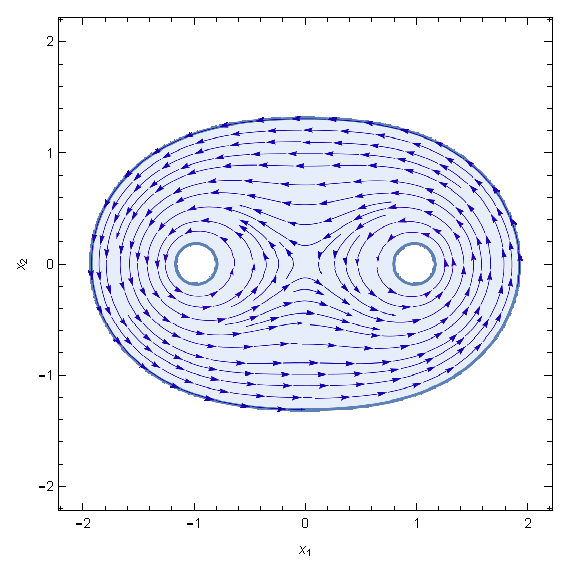
\includegraphics[width=0.6\textwidth]{../Plots/HarmonicVectorFields_gr1.eps}
  \caption{A plot of $u=\nabla^\perp\psi$ in the region $\psi^{-1}\brk*{[-1,1]}$.
    Here $\psi$ is given by equation \eqref{eq:n2:hvf:noInflowNoOutflow}.}
  \label{pl:n2_hvf_noInflowNoOutflow}
\end{figure}
Since $\psi$ is constant on each component of $\partial X$ the function $u$ has 
no inflow or outflow.
It follows from $\psi(-x)=\psi(x)$ that $u(-x)=-u(x)$ 
and thus the origin $x=0$ is a stagnation point.
By proposition \ref{pr:n2_hvf_noInflowNoOutflow} it is in fact the
sole stagnation point of $u$ on $X$.

In a second example from \cite{Wahlen2023} we fix the domain rather than the function.
For this set $X=\overline{B_4}\setminus\brk*{B_1(2e_1)\cup B_1(-2e_1)}$ to be the domain.
We then have the system
\begin{equation}
  \begin{aligned}
    \Delta \psi&=0 &&\text{, on }\Omega \\
    \psi&=0 &&\text{, on the outer ring }4S^1 \\
    \psi&=1 &&\text{, on the inner rings }S^1(-2e_1)\cup S^1(2e_1)
  \end{aligned}\label{eq:n2:hvf:roundRegion:noInflowNoOutflow}
\end{equation}
We solve this system numerically and set $u=\nabla^\perp\psi$.
The result is plotted in figure \ref{pl:n2_hvf_roundRegion_noInflowNoOutflow}.
\begin{figure}
  \centering
  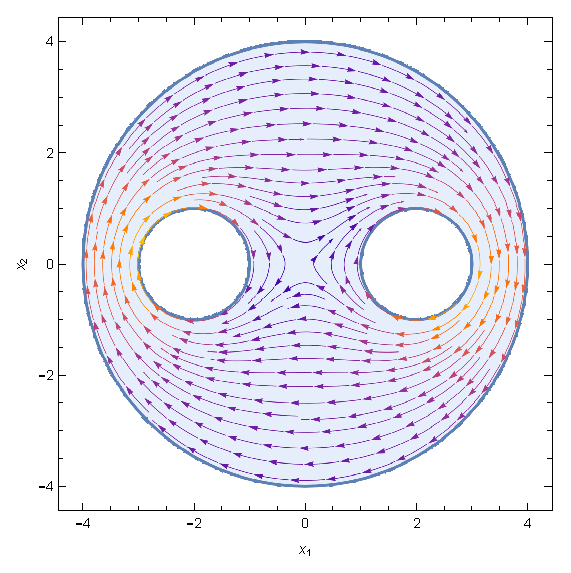
\includegraphics[width=0.6\textwidth]{../Plots/HarmonicVectorFields_gr4.eps}
  \caption{A plot of $u=\nabla^\perp\psi$ where $\psi$ is the numerical solution to
   \eqref{eq:n2:hvf:roundRegion:noInflowNoOutflow}.}
  \label{pl:n2_hvf_roundRegion_noInflowNoOutflow}
\end{figure}
Again it follows from symmetry that the origin is a stagnation point and
from proposition \ref{pr:n2_hvf_noInflowNoOutflow} that it is in fact the sole stagnation point of $u$.

\section{Example of inflow on one side and outflow on the other}
In the following we aim to give examples of domains in $d=2$ dimensions for which 
we have inflow on one simply connected boundary component and outflow on another simply connected boundary
component with stagnation points.
For this consider first the stream function
\begin{equation}
  \begin{aligned}
  \psi\colon \R^2\setminus\brk[c]*{-e_1,e_1}&\to\R \\
  x&\mapsto\Phi_2\brk*{x-e_1}+x_1
  \end{aligned}\label{eq:n2:hvf:InflowOutflow:singleHole}
\end{equation}
Figure \ref{pl:n2_hvf_InflowOutflow_asymmetric_single} indicates that $u=\nabla^\perp\psi$ fulfils the
requirements on the domain $X=\psi^{-1}\brk*{[-0.5,2]}\cap \R\times[-2,2]$.
\begin{figure}
  \centering
  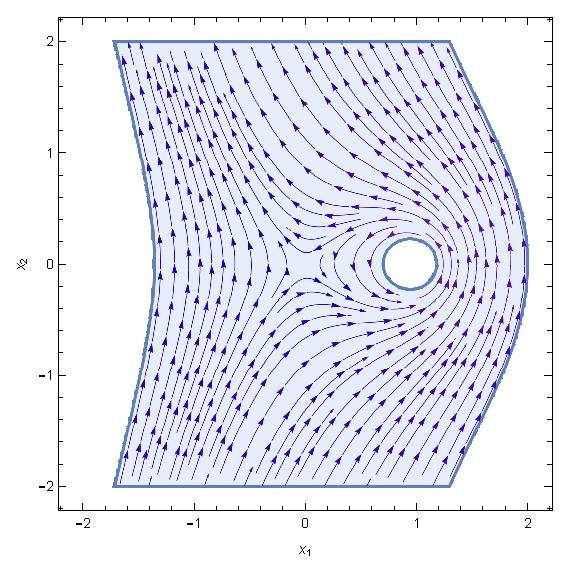
\includegraphics[width=0.6\textwidth]{../Plots/HarmonicVectorFields_gr3.eps}
  \caption{A plot of $u=\nabla^\perp\psi$ in the region $\psi^{-1}\brk*{[-0.5,2]}\cap \R\times[-2,2]$.
  Here $\psi$ is given by equation \eqref{eq:n2:hvf:InflowOutflow:singleHole}.}
  \label{pl:n2_hvf_InflowOutflow_asymmetric_single}
\end{figure}
An elementary calculation reveals that the origin is a stagnation point of $u$.

Now we would like to have a harmonic vector field similar to the example with two holes with
inflow on the one side and outflow on the other. 
For this consider the streamline
\begin{equation}
  \begin{aligned}
  u\colon\R^2\setminus\brk[c]*{-e_1,e_1}&\to\R \\
  x&\mapsto\Phi_2\brk*{x-e_1}-\Phi_2\brk*{x+e_1}+x_1
  \end{aligned}\label{eq:n2:hvf:noInflowNoOutflow:doubleHoles}
\end{equation}
Figure \ref{pl:n2_hvf_InflowOutflow_symmetric_region} indicates that $u=\nabla^\perp\psi$ 
on the domain $X=\psi^{-1}\brk*{[-0.7,0.7]}\cap \R\times[-2,2]$ is the function
we are looking for.
\begin{figure}
  \centering
  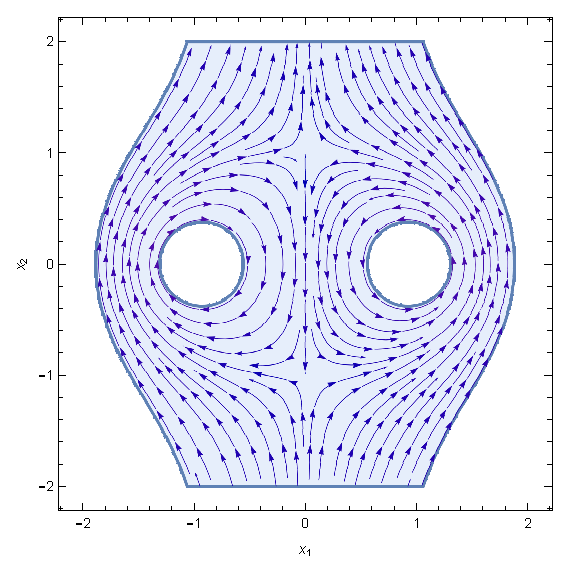
\includegraphics[width=0.6\textwidth]{../Plots/HarmonicVectorFields_gr2.eps}
  \caption{A plot of $u=\nabla^\perp\psi$ in the region $\psi^{-1}\brk*{[-0.7,0.7]}\cap \R\times[-2,2]$.
  Here $\psi$ is given by equation \eqref{eq:n2:hvf:noInflowNoOutflow:doubleHoles}.}
  \label{pl:n2_hvf_InflowOutflow_symmetric_region}
\end{figure}


In another example given by \cite{Wahlen2023} we fix the domain rather than the function.
Let $\Omega=B_4\setminus\brk*{B_1(2e_1)\cup B_1(-2e_1)}$ be the domain as before.
We now have the system
\begin{equation}
  \begin{aligned}
    \Delta \psi&=0 &&\text{, on }\Omega \\
    \psi&=0 &&\text{, on the outer ring }4S^1 \\
    \psi&=-1 &&\text{, on the left inner ring }S^1(-2e_1) \\
    \psi&=1 &&\text{, on the right inner ring }S^1(2e_1)
  \end{aligned}\label{eq:n2:hvf:roundRegion:InflowOutflow}
\end{equation}
We solve this system numerically and set $u=\nabla^\perp\psi$.
The result is plotted in figure \ref{pl:n2_hvf_roundRegion_InflowOutflow}.
\begin{figure}
  \centering
  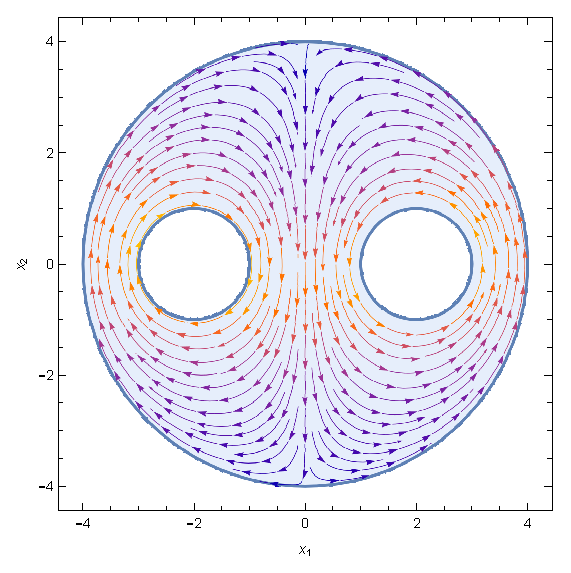
\includegraphics[width=0.6\textwidth]{../Plots/HarmonicVectorFields_gr5.eps}
  \caption{A plot of $u=\nabla^\perp\psi$ where $\psi$ is the numerical solution to
   \eqref{eq:n2:hvf:roundRegion:InflowOutflow}.}
  \label{pl:n2_hvf_roundRegion_InflowOutflow}
\end{figure}
Here we obtain from the symmetry $\psi(-x_1,x_2)=\psi(x)$ that $\psi=0$ on
the $x_2$-axis. Since also $\psi=0$ on $4S^1$ we have two stagnation points
at $\pm4e_2$.

\chapter{Harmonic functions, $d=3$}

\section{The cylinder}

The following proof comes from \cite{Wahlen2023}
\begin{proposition}
  Let $\Omega=(0,1)\times U\subseteq\R^3$ be an open cylinder where $U\subseteq\R^2$ is an open set.
  Let further $f\colon X=\overline{\Omega}\to\R$ be
  harmonic such that the sides
  $[0,1]\times \partial U=\Sigma^0$ are the tangential boundary,
  the lid $\brk[c]{0}\times U=\Sigma^+$ is the entrant boundary and
  the lid $\brk[c]{1}\times U=\Sigma^-$ is the emergent boundary. 
  Then $f$ cannot have an interior critical point.
\end{proposition}
\begin{proof}
  Assume not. Since
  \begin{align*}
    \Delta(\partial_1f)=\partial_1(\Delta f)=0
  \end{align*}
  we have by the maximum principle that $\partial_1 f$ attains its minimum on the boundary $\Sigma$. Since $\partial_1 f(x)=0$ for some interior point 
  by assumption and $\partial_1 f>0$ on the lids $\brk[c]{x_1=0}\cup\brk[c]{x_1=1}$ there exists a point
  $x\in(0,1)\times \partial U$ such that $\partial_1f(x)$ is minimal on $X$. But then we have by Hopf's lemma
  that
  \begin{align*}
    0<\nabla (\partial_1f)\cdot n=\partial_1(\nabla f\cdot n)=0\,,
  \end{align*}
  a contradiction.
\end{proof}

\section{Simply connected entrant boundary}

Mimicking the proof in 2 dimensions we obtain the following proposition.
\begin{proposition}
  Let $X\subset\R^3$ be a compact manifold homeomorphic to the ball $B$ such that $\Sigma$ is a differentiable manifold.
  Let $f\colon X\to\R$ be a Morse harmonic function. Assume that the strictly entrant boundary $\Sigma^-$ is non-empty and simply connected.
  Then we have that
  \begin{align*}
    M_1-M_2=0\,.
  \end{align*}
\end{proposition}
\begin{proof}
  As in the two dimensional case we split the domain $\Omega$ with a surface $\Gamma$ such that
  $\partial\Gamma=\gamma=\partial\Sigma^-$.
  \td{Why would this even be possible?}
  Denote the two arising domains $X^+$ and $X^-$ where $\partial X^-\cap\Sigma^+\subseteq\gamma$ and
  $\partial X^+\cap \Sigma^-\subseteq\gamma$.
  We can assume that $\Gamma$ as well as $\gamma$ are smooth manifold.
  Since by proposition \ref{pr:finiteness_critical_points} there are finitely many interior critical points in $X$
  we can also assume that no interior critical points lie on $\Gamma$.
  Furthermore we assume that $\Gamma$ is bent towards $X^+$ at $\gamma$.
  For the following argumentation we require that $f$ is strongly Morse on both $X^+$ and
  $X^-$ so assume for a moment that this is the case.
  Now we have that $\gamma$ is homeomorphic to the circle $\R/\Z$.
  Since $f$ is non-degenerate the
  the number of maxima and minima of $f$ on $\gamma$ must be equal and thus
  \begin{align}
    \ind_{\gamma^+,0}(f)+\ind_{\gamma^-,1}(-f)=\ind_{\gamma^+,1}(f)+\ind_{\gamma^-,0}(-f)
    \label{eq:n3_disproof_morse_maxMinRel}
  \end{align}
  % \begin{align}
  %   \ind_{\gamma^+,0}(f)+\ind_{\gamma^-,1}(-f)=2l
  % \end{align}
  % for some $l\in\N$.\ruggedtodo{elaborate this}
  We now turn our attention to $X^+$. Since no essential critical points lie on $\Sigma^+$ 
  it follows for the boundary type numbers that
  \begin{align}
    \mu^+_k=\ind_{\Gamma^+,k}(f)+\ind_{\gamma^+,k}(f)\,.\label{eq:n3_disproof_morse_muplus}
  \end{align}
  Analogously we have on $X^-$ that
  \begin{align}
    \nu^-_k=\ind_{\Gamma^-,k}(-f)+\ind_{\gamma^-,k}(-f)\,.\label{eq:n3_disproof_morse_numinus}
  \end{align}
  In addition we have that the emergent critical points on $\Gamma=\Gamma^+$ of $f$ on $X^+$ are the
  entrant critical points on $\Gamma=\Gamma^-$ of $-f$ on $X^-$, that is
  \begin{equation}
    \begin{aligned}
      \ind_{\Gamma^+,0}(f)&=\ind_{\Gamma^-,2}(-f) \\
      \ind_{\Gamma^+,1}(f)&=\ind_{\Gamma^-,1}(-f) \\
      \ind_{\Gamma^+,2}(f)&=\ind_{\Gamma^-,0}(-f)\label{eq:n3_disproof_morse_relationIndex} 
    \end{aligned}\,.
  \end{equation}
  Using equations \eqref{eq:n3_disproof_morse_muplus}, \eqref{eq:n3_disproof_morse_numinus} and \eqref{eq:n3_disproof_morse_relationIndex}
  we obtain
  \begin{equation}
    \begin{aligned}
      \mu^+_0-\nu^-_2&=\ind_{\gamma^+,0}(f) \\
      \mu^+_1-\nu^-_1&=\ind_{\gamma^+,1}(f)-\ind_{\gamma^-,1}(-f) \\
      \mu^+_2-\nu^-_0&=-\ind_{\gamma^-,0}(-f)
    \end{aligned}\,.\label{eq:n3_disproof_morse_relationMuNu}
  \end{equation}
  We observe the Morse inequalities for $f$
  \begin{align}
    M_2^++\mu^+_2-M_1^+-\mu^+_1+\mu^+_0=\chi(X^+)=\chi(X)\,.\label{eq:n3_disproof_morse_morseineqplus}
  \end{align}
  and the Morse inequalities for $-f$
  \begin{align}
    M_1^-+\nu^-_2-M_2^--\nu^-_1+\nu^-_0=\chi(X^-)=\chi(X)\label{eq:n3_disproof_morse_morseineqminus}
  \end{align}
  where the $M_k$ continue to denote the interior type numbers of $f$.
  We now subtract equation \eqref{eq:n3_disproof_morse_morseineqminus} from \eqref{eq:n3_disproof_morse_morseineqplus}
  and insert relations \eqref{eq:n3_disproof_morse_relationMuNu} to obtain
  then with equation \eqref{eq:n3_disproof_morse_maxMinRel}
  \begin{align*}
    0&=M_1^--M_2^-+M_1^+-M_2^++\ind_{\gamma^+,0}(f)+\ind_{\gamma^-,1}(-f)-\ind_{\gamma^+,1}(f)-\ind_{\gamma^-,0}(-f) \\
    &= M_1-M_2
  \end{align*}
  from which the claim follows.

  The claim remains to be shown in the case that $f$ is not strongly Morse on $X^+$ and $X^-$. In this case let
  $f^\e$ for $\e\in E$ be a family of strongly Morse functions as in corollary \ref{co:density_boundaryGeneric}.
  Since $x_1$, $x_2$ are non-degenerate critical points of $f$
  due to the slanted angle at which
  $\Gamma$ approaches $\gamma$
  we obtain that
  \begin{align}
    \ind_{\gamma,k}\brk*{f^\e}=\ind_{\gamma,k}(f)\qquad\text{ and }\qquad 
    \ind_{\gamma,k}\brk*{-f^\e}=\ind_{\gamma,k}(-f)
    \label{eq:n3_disproof_morse_indexApprox}
  \end{align}
  By the same corollary we can assume that $f^\e$ has no essential critical points on
  $\Sigma^+(f)$ and $-f^\e$ has no essential critical points on $\Sigma^-(f)$.
  The claim then follows by the calculations above where we replace
  $f$ with $f^\e$ and then note that $M_1^\e=M_1$ and $M_2^\e=M_2$.
\end{proof}


\section{A harmonic function with interior critical point and simply connected entrant boundary}
In fact we can give an example for such a function with
simply connected entrant boundary.
\begin{example}[A harmonic function with interior critical point and simply connected entrant boundary]
  Consider the domain $X=\overline{B}_r\subseteq\R^3$ with $r>0$ sufficiently large and the harmonic function
  \begin{align*}
    f\colon X&\to\R \\
    x&\mapsto \frac{x_1^2}{2}-\frac{x_1^3}{3}-\frac{x_2^2}{2}+x_1x_2^2+x_2x_3
  \end{align*}
  This induces the harmonic vector field
  \begin{align*}
    u\colon X&\to\R^3 \\
    x&\mapsto\vect{x_1(1-x_1)+x_2^2 \\
      x_2(2x_1-1)+x_3 \\
      x_2}
  \end{align*}
  It follows from setting $u(x)=0$ implies that $x_2=0$
  and then that $x_3=0$ and $x_1\in\brk[c]*{0,1}$. Thus we have that $x\in\brk[c]*{0,e_1}$
  are the sole possible zeroes of $u$. Conversely these are zeroes of $u$.

  Figure \ref{pl:n3_hf_inflowOutflowStagnationPoint_overview}
  indicates that $f$ has the desired properties.
  \begin{figure}
    \centering
    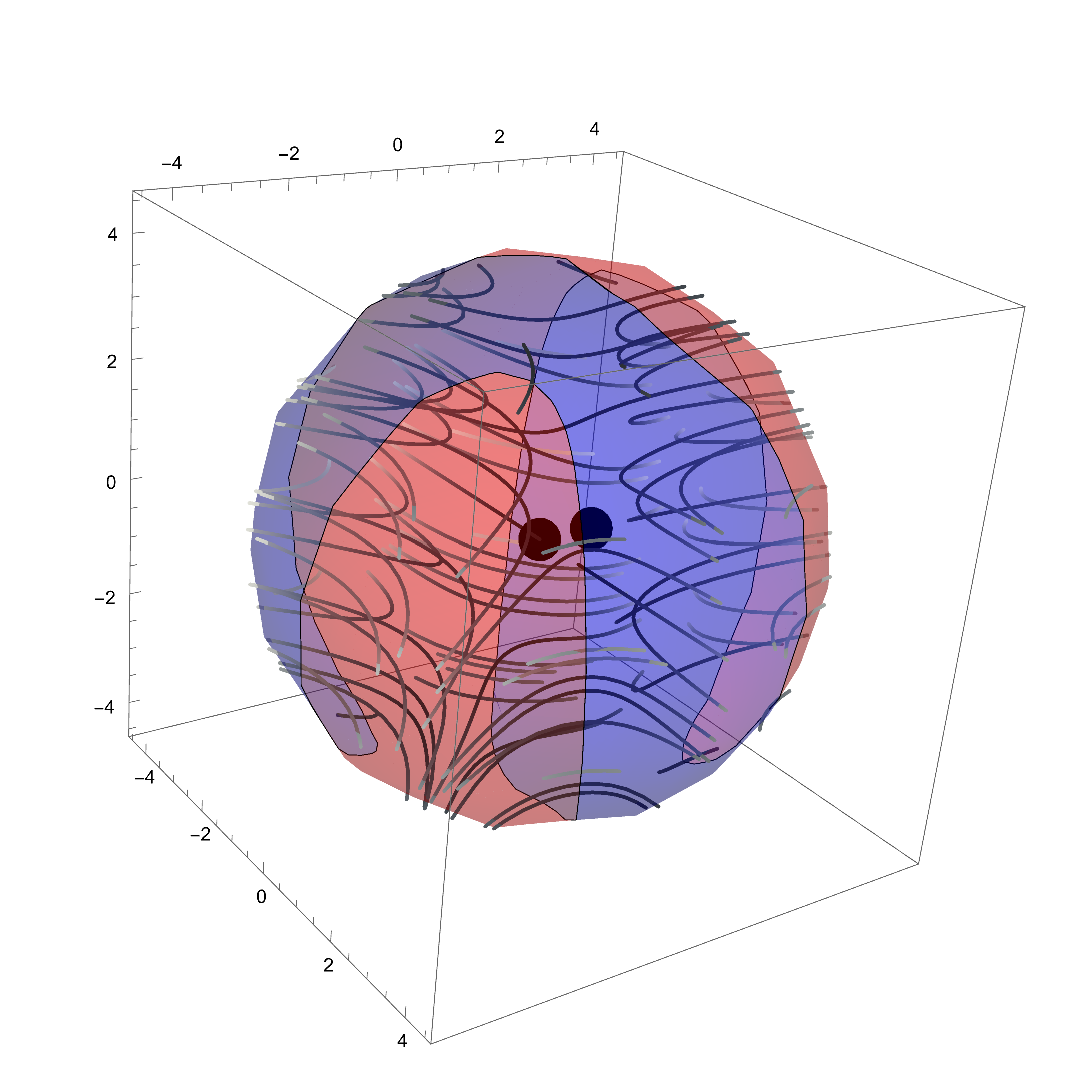
\includegraphics[width=0.6\textwidth]{../plots/n3_hf_inflowOutflow_Ball_overview.pdf}
    \caption{A plot of the function $u$}
    \label{pl:n3_hf_inflowOutflowStagnationPoint_overview}
  \end{figure}
  \begin{figure}
    \centering
    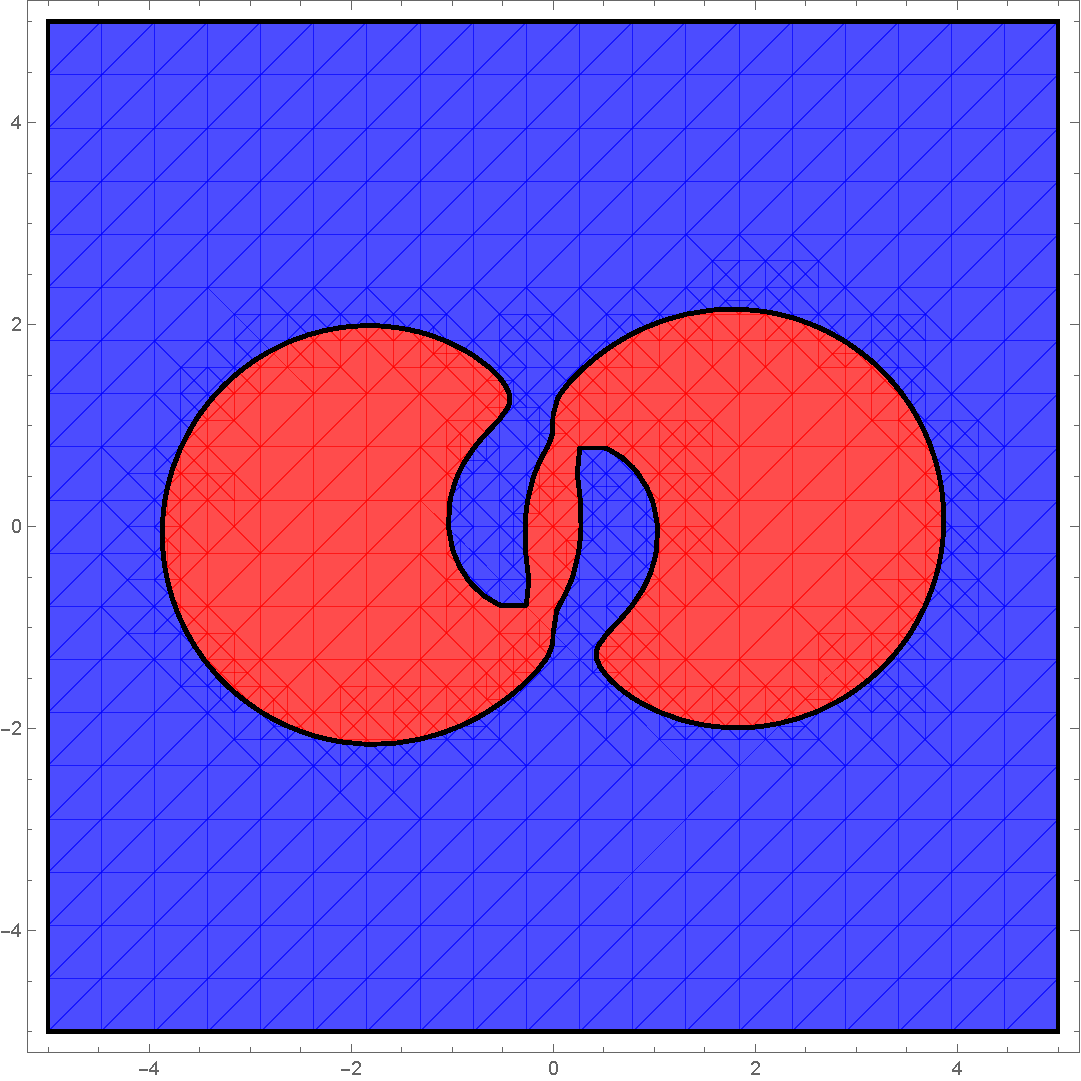
\includegraphics[width=0.6\textwidth]{../plots/n3_hf_inflowOutflow_Ball_Surface.pdf}
    \caption{Stereographic projection of the surface $\Sigma$.}
    \label{pl:n3_hf_inflowOutflowStagnationPoint_Surface}
  \end{figure}
\end{example}
\begin{proposition}
  The function given by equation \eqref{} has simply connected emergent and entrant boundaries.
\end{proposition}
\begin{proof}
  Consider the inverse stereographic projection given by 
  \begin{align*}
    \psi\colon \R^2&\to B_r\setminus\brk[c]*{re_1} \\
    x&\mapsto \frac{r}{s^2+1}\vect{s^2-1 \\ x}
  \end{align*}
  where $s=\abs{x}$. We calculate
  \begin{align*}
    rn\cdot u(x) = x_1^2(1-x_1)+x_2^2(3x_1-1)+2x_2x_3
  \end{align*}
  If we precompose with the inverse stereographic projection we obtain
  \begin{align*}
    &\brk*{rn\cdot u}\circ\psi (x) \\
    &= \frac{r^2}{\brk*{s^2+1}^3}\brk*{\brk*{s^2-1}^2\brk*{\brk*{s^2+1}-r\brk*{s^2-1}}+x_1^2\brk*{3r\brk*{s^2-1}-\brk*{s^2+1}}+2x_1\brk*{s^2+1}x_2}
  \end{align*}
  which vanishes precisely iff
  \begin{align*}
    0&=\frac{1}{r}\brk*{s^2-1}^2\brk*{\brk*{s^2+1}-\brk*{s^2-1}}+x_1^2\brk*{3\brk*{s^2-1}-\frac{1}{r}\brk*{s^2+1}}+\frac{1}{r}2x_1\brk*{s^2+1}x_2 \\
    &=\frac{1}{r}\brk*{s^2+1}\brk*{\brk*{s^2-1}^2-x_1^2}-\brk*{s^2-1}^3+3\brk*{s^2-1}x_1^2+\frac{1}{r}2x_1x_2\brk*{s^2+1}
  \end{align*}
  Writing $\e=1/r$ and setting
  \begin{align*}
    p^\e(x)=\e\brk*{\brk*{s^2+1}\brk*{\brk*{s^2-1}^2-x_1^2}+2x_1x_2\brk*{s^2+1}}-\brk*{s^2-1}^3+3\brk*{s^2-1}x_1^2
  \end{align*}
  we see that this is equivalent to the condition $p^\e(x)=0$.
  Our aim is to show that the real planar variety defined in this way is compact and has precisely one connectivity component.
  It then follows from the Jordan curve theorem that this variety splits the plane into two components, namely one where 
  $p^\e$ is positive and one where it is negative. The image of these sets under the stereographic projection is then precisely
  $\Sigma^+$ and $\Sigma^-$ respectively and it follows that these sets are simply connected.

  % we also calculate for this part
  % \begin{align*}
  %   \nabla q_1(x)=2\vect{3x_1^2x_2 + x_1x_2^2 + x_2^3 - x_1 + x_2 \\ x_1^3 + x_1^2x_2 + 3x_1x_2^2 + 2x_2^3 + x_1}
  % \end{align*}
  % and
  % \begin{align*}
  %   D^2q_1(x)=2\begin{bmatrix}
  %     6x_1x_2 + x_2^2 - 1 & 3x_1^2 + 2x_1x_2 + 3x_2^2 + 1 \\
  %     *& x_1^2 + 6x_1x_2 + 6x_2^2
  %   \end{bmatrix}
  % \end{align*}
  % Now notice that we have around the point $\pm e_2$ that
  % \begin{align*}
  %   D^2q_1(\pm e_2)=2\begin{bmatrix}
  %     0 & 4 \\
  %     4 & 6
  %   \end{bmatrix}
  % \end{align*}
  % which is of full rank. 


  % \begin{align*}
  %   \psi\colon \R^2&\to B_r\setminus\brk[c]*{re_3} \\
  %   x&\mapsto \frac{r}{s^2+1}\vect{x \\ s^2-1}
  % \end{align*}
  % where $s=\abs{x}$. We calculate
  % \begin{align*}
  %   rn\cdot u(x) = x_1^2(1-x_1)+x_2^2(3x_1-1)+2x_2x_3
  % \end{align*}
  % If we now precompose with the inverse stereographic projection we obtain
  % \begin{align*}
  %   &\brk*{rn\cdot u}\circ\psi (x) \\
  %   &= \frac{r^2}{\brk*{s^2+1}^3}\brk*{x_1^2\brk*{\brk*{s^2+1}-rx_1}+x_2^2\brk*{3rx_1-\brk*{s^2+1}}+2x_2\brk*{s^2+1}\brk*{s^2-1}}
  % \end{align*}
  % which vanishes precisely iff
  % \begin{align}
  %   0&=x_1^2\brk*{\brk*{s^2+1}-rx_1}+x_2^2\brk*{3rx_1-\brk*{s^2+1}}+2x_2\brk*{s^2+1}\brk*{s^2-1} \\
  %   &=\brk*{s^2+1}\brk*{x_1^2-x_2^2}-rx_1^3+3rx_1x_2^2+2x_2\brk*{s^4-1}
  % \end{align}
\end{proof}

\begin{proposition}
  There exists an $\e>0$ such that the planar variety $p^\e(x)$ given by equation \eqref{}
  has one connectivity component.
\end{proposition}
\begin{proof}
  By proposition \ref{pr:n3_polynomial_Vp0} we have that $V\brk*{p^0}$
  consists of six arcs which all meet at the points $e_2$ and $-e_2$.
  The set $V\brk*{p^0}$ is sketched in figure \ref{}.
  We will argue that the corresponding figure for a small enough $\e$ is given by \ref{}.
  Away from the singularities at $\pm e_2$ we obtain the result by proposition \ref{} and picking
  $\e$ small enough. By symmetry of $p^\e$, that is we have
  \begin{align}
    p^\e\brk*{-x}=p^\e(x)
  \end{align}
  it suffises to inspect what happens around the point $e_2$ as $\e\to0$.

  Now define the polynomial $q$ by
  \begin{align}
    p^\e(x)=\e q(x)+p^0(x)\,.
  \end{align}
  For simplicity we would like to move the singular point to the origin so we give
  \begin{align*}
    p^0(x-e_2)=(x_1^2 + x_2^2 - 2x_2)(x_1^4 + 2x_1^2x_2^2 + x_2^4 - 4x_1^2x_2 - 4x_2^3 - 3x_1^2 + 4x_2^2)
  \end{align*}
  and
  \begin{align*}
    q(x-e_2)=(x_1^2 + x_2^2 - 2x_2 + 2)(2x_1x_2 + x_2^2 - 2x_1 - 2x_2)
  \end{align*}
  By Tougeron's theorem there exists a neighbourhood $U$ around the origin such that
  \begin{align}
    p\colon (\e,x)\mapsto p^\e(x)
  \end{align}
  % is diffeomorphic on $U$ to its jet
  % \begin{align}
  %   J^{}
  % \end{align}
  \td{continue this argument}
  Taking the homogeneous parts of lowest order we obtain
  \begin{align*}
    h_3(x)=\brk*{p^0\brk*{x-e_2}}_3=2x_2(3x_1^2-4x_2^2)
  \end{align*}
  and
  \begin{align*}
    h_1(x)=\brk*{q\brk*{x-e_2}}_1=-4(x_1+x_2)\,.
  \end{align*}
  % We now denote the arcs $\alpha_k$ as in the plot \ref{}.
  % \td{insert plot}
  % \begin{figure}
  %   \centering
  %   \missingfigure[]{}
  %   \caption{Plot of $\brk*{p^0\brk*{x-e_2}}_3$}
  % \end{figure}
  % We claim that for $\e$ sufficiently small the function
  In proposition \ref{pr:n3_polynomial_regularH}
  it will be shown that the polynomial
  \begin{align}
    h^\e(x)=\e h_1(x)+h_3(x)\,.
  \end{align}
  has a variety of the shape given in figure \ref{fi:n3_polynomial_intersectionOriginRegular}
  % is obtained by removing the singular point and adding handles between
  % the arcs $\alpha_2$ and $\alpha_5$, $\alpha_3$ and $\alpha_4$ and $\alpha_6$ and $\alpha_1$.
  % To see this note that
  Moreover $V\brk*{h^\e}$ converges to $V\brk*{h^0}$ with respect to the Hausdorff metric as
  $\e\to0$. Now 
  \td{continue proof}
\end{proof}

% Let $p\in\R\pwrSeries{X_1,\dots,X_n}$ be a formal power series.
% The following definitions are inspired by \cite{Viro2006}.
% Define the \emph{Milnor number} $m\brk*{p}$ as the dimension
% \begin{align}
%   m\brk*{p}= \dim_\R\bigslant{\R\pwrSeries{X_1,\dots,X_n}}{\brk*{\partial_1p,\dots,\partial_np}}
% \end{align}
% where $\brk*{\partial_1p,\dots,\partial_np}$ denotes the ideal spanned by the
% partial derivatives of $p$.

% \begin{theorem}[Tougeron's theorem]
%   If $x$ is a singularity of $V\brk*{p}$ with finite Milnor number $m$
%   then there exists a neighbourhood $U$ of $x$ and a diffeomorphism
%   \begin{align}
%     \phi\colon U\to \phi(U)
%   \end{align}
%   such that
%   \begin{align}
%     \phi\brk*{V_U\brk*{p}}=V_{\phi(U)}\brk*{J^{m+1}_xp}
%   \end{align}
%   where $J^{m+1}_x p$ is the $m+1$-jet of $p$ at $x$.
% \end{theorem}
% \begin{proof}
%   See \cite{Arnold2012}.
% \end{proof}

\begin{proposition}[The set $V\brk*{p^0}$]\label{pr:n3_polynomial_Vp0}
  The set $V\brk*{p^0}$ where $p^0$ given by equation \eqref{}
  consists of six arcs which all meet at the points $\pm e_2$ and nowhere else.
\end{proposition}
\begin{proof}
  \tdrewrite{It should be much easier arguing in $\R^3$.}
  From the factorisation
  \begin{align*}
    p^0(x)=\underbrace{\brk*{s^2-1}}_{=q_1(x)}\underbrace{\brk*{\brk*{s^2-1}^2-3x_1^2}}_{=q_2(x)}
  \end{align*}
  we see that
  \begin{align*}
    V\brk*{p^0}=V\brk*{q_1}\cup V\brk*{q_2}=S^1\cup V\brk*{q_2}
  \end{align*}
  We claim that the set of points $V\brk*{q_2}$ consists of four curves intersecting the
  circle $S^1$ precisely at the points $\pm e_2$ and that there are no other singular points.
  From this the claim will then follow.
  To show this take a closer look at
  \begin{align*}
    q_2(x)=\brk*{s^2-1}^2-3x_1^2\,.
  \end{align*}
  Substituting $\tix_k=x_k^2$ we can write this as
  \begin{align*}
    q_2(x)&=\brk*{\tix_1+\tix_2-1}^2-3\tix_1\\
    &=\tix_1^2+2\tix_1\tix_2+\tix_2^2-5\tix_1-2\tix_2+1 \\
    &=\brk*{\tix_1+\tix_2}^2-5\tix_1-2\tix_2+1\\
    &=\tiq_2\brk*{\tix}\,.
  \end{align*}
  Now the equation 
  \begin{align*}
    0=\tiq_2\brk*{\tix}
  \end{align*}
  is that of a conic section. Since we are assuming $\tix\in\R_{\geq0}^2$
  we obtain the connected arc $\tiA$ in the upper right quadrant intersecting the $\tix_1$-axis at the points
  \begin{align*}
    \tia^\pm=\vect{\frac{5\pm2\sqrt{6}}{2} & 0}^\top
  \end{align*}
  and touching the $\tix_2$-axis at the point $e_2$.
  The arc $\tiA$ is shown in figure \ref{fi:n3_polynomial_conicArc}.
  \begin{figure}
    \centering
    \input{../Figures/n3_polynomial_conicArc.pdf_tex}
    \caption{The arc $\tiA$.}
    \label{fi:n3_polynomial_conicArc}
  \end{figure}
  Since there are only two points where the curve intersects $\partial\R_{\geq0}^2$
  and the curve does not leave this quadrant at infinity it follows that $\tiC$ is
  a connected compact arc.
  Define the mappings
  \begin{align}
    \sqrt[\leftroot{2}\uproot{4}\circ_1\circ_2]{}\colon \R_{\geq0}^2&\to\R^2 \\
    \tix&\mapsto x=\vect{\circ_1\sqrt{\tix_1}&\circ_2\sqrt{\tix_2}}^\top
  \end{align}
  for signs $\circ_1,\circ_2\in\brk[c]*{+,-}$.
  Now taking the image of the arc $\tiA$ under this square root we obtain four arcs
  \begin{align*}
    A^{\circ_1\circ_2}=\brk[c]*{\sqrt[\leftroot{2}\uproot{4}\circ_1\circ_2]{\tix}\colon\tix\in \tiA}
  \end{align*}
  for signs $\circ_1,\circ_2\in\brk[c]*{+,-}$.
  Note that by construction the arc $A^{++}$ lies in the first quadrant and analogously
  $A^{-+}$, $A^{--}$ and $A^{+-}$ lie in the second, third and fourth quadrants.
  Now define four points on the $x_1$-axis by
  \begin{align}
    a^{\circ_1\circ_2}=\sqrt[\leftroot{2}\uproot{4}\circ_1+]{a^{\circ_2}}\,.
  \end{align}
  We see that $A^{++}\cap A^{+-}=\brk[c]*{a^{++},a^{+-}}$ and
  $A^{-+}\cap A^{--}=\brk[c]*{a^{--},a^{-+}}$.
  We also see that $A^{++}\cap A^{-+}=\brk[c]*{e_2}$ and 
  $A^{--}\cap A^{+-}=\brk[c]*{-e_2}$
  Since the origin is not contained in any arc it thus follows that $A^{++}\cap A^{--}=\emptyset$ 
  and $A^{-+}\cap A^{+-}=\emptyset$.
  Thus the union
  \begin{align}
    A=A^{++}\cup A^{+-}\cup A^{-+}\cup A^{--}
  \end{align}
  consists of four arcs which meet at the points $\pm e_2$ and hence also
  $V\brk*{p_2}=A$.

  It now remains to be shown that $A\cap S^1=\brk[c]*{\pm e_2}$.
  For this let $x\in S^1$ such that
  \begin{align}
    0=q_2(x)
  \end{align}
  but then this claim follows immediately from $q_2(x)=-3x_1^2$.

  \begin{figure}
    \centering
    \input{../Figures/n3_polynomial_projectionComponentConics.pdf_tex}
    \caption{Sketch of the set $V\brk*{q_2}$.}
    \label{fi:n3_polynomial_projectionComponentConics}
  \end{figure}
  

%   Since we have that
%   \begin{align*}
%     q(x)=\brk*{x_1^2+x_2^2}^2-3x_1^2
%     =x_1^4+x_2^4+2x_1^2x_2^2-3x_1^2
%   \end{align*}
%   has the gradient
%   \begin{align*}
%     \nabla q(x)=\vect{4x_1^3+4x_1x_2^2-6x_1 \\ 4x_2^3+4x_1^2x_2}
%     =4\vect{x_1\brk*{x_1^2+x_2^2-\frac{3}{2}x_1} \\ x_2^3+x_1^2x_2}
%   \end{align*}
%   which does not vanish at the points given by \eqref{eq:n3_example_rootsOfZeroes}
%   we have that the four curves are in fact two curves.
%   We also calculate the derivative
%   \begin{align*}
%     \nabla p^0(x)=\vect{}
%   \end{align*}
%   and the second derivative
%   \begin{align*}
%     D^2p^0(x)=6\begin{bmatrix}
%       5x_1^4 + 6x_1^2x_2^2 + x_2^4 - 12x_1^2 - 3x_2^2 + 2 & 2x_1x_2(2x_1^2 + 2x_2^2 - 3) \\
%       * & x_1^4 + 6x_1^2x_2^2 + 5x_2^4 - 3x_1^2 - 6x_2^2 + 1
%     \end{bmatrix}
%   \end{align*}
%   Note that this is degenerate at the points $\pm e_2$.
  
%   All six curves intersect precisely at the points $\pm e_1$. If we now add the variation
%   \begin{align*}
%     q_1(x)=\brk*{s^2+1}\brk*{\brk*{s^2-1}^2-x_1^2}+2x_1x_2\brk*{s^2+1}
%   \end{align*}
%   to our variety we 
\end{proof}

\begin{proposition}
  For $\e>0$ sufficiently small the variety $V\brk*{p^\e}$ is smooth.
\end{proposition}
\begin{proof}
  % Since we \emph{really} do not want to deal with sixth order polynomials we take the stereographic
  % projection when constructing $p^\e$ in a different component to obtain a fifth order polynomial instead
  % (much better). For this let
  % \begin{align*}
  %   \psi\colon \R^2&\to B_r\setminus\brk[c]*{re_3} \\
  %   x&\mapsto \frac{r}{s^2+1}\vect{x \\ s^2-1}
  % \end{align*}
  % where $s=\abs{x}$. 
  % If we now precompose with this new inverse stereographic projection we obtain
  % \begin{align*}
  %   &\brk*{rn\cdot u}\circ\psi (x) \\
  %   &= \frac{r^2}{\brk*{s^2+1}^3}\brk*{x_1^2\brk*{\brk*{s^2+1}-rx_1}+x_2^2\brk*{3rx_1-\brk*{s^2+1}}+2x_2\brk*{s^2-1}\brk*{s^2+1}}
  % \end{align*}
  % which vanishes precisely iff
  % \begin{align}
  %   0&=2x_1^4x_2+4x_1^2x_2^3+2x_2^5+x_1^4-x_2^4-rx_1^3+3rx_1x_2^2+x_1^2-x_2^2-2x_2=P^r(x)
  % \end{align}
  % In order to show smoothness it is sufficient 
  % to show that $V\brk*{P^r,\partial_1P^r,\partial_2P^r}=\emptyset$.
  % Thus we calculate
  % \begin{align}
  %   \partial_1P^r(x)
  %   &=8x_1^3x_2+8x_1x_2^3+4x_1^3-3rx_1^2+3rx_2^2+2x_1
  % \end{align}
  % and
  % \begin{align}
  %   \frac{1}{2}\partial_2P^r(x)
  %   &=x_1^4+6x_1^2x_2^2+5x_2^4-2x_2^3+3rx_1x_2-x_2-1
  % \end{align}
  % We further obtain
  % \begin{align}
  %   \frac{x_1}{2}\partial_1P^r(x)
  %   &=4x_1^4x_2+4x_1^2x_2^3+2x_1^4-\frac{3}{2}rx_1^3+\frac{3}{2}rx_2^2x_1+x_1^2
  % \end{align}
  % and
  % \begin{align}
  %   x_2\partial_2P^r(x)
  %   &=2x_1^4x_2+12x_1^2x_2^3+10x_2^5-4x_2^4+6rx_1x_2^2-2x_2^2-2x_2
  % \end{align}
  % and thus
  % \begin{align}
  %   &P^r(x)-\frac{x_1}{2}\partial_1P^r(x)-x_2\partial_2P^r(x) \\
  %   &=-4x_1^4x_2+2x_2^5-x_1^4-x_2^4+\frac{1}{2}rx_1^3+\frac{3}{2}rx_1x_2^2-x_2^2-2x_2
  % \end{align}
  % \begin{align}
  %   &P^r(x)-x_2\partial_2P^r(x) \\
  %   &=-2x_1^4x_2+x_1^4-x_2^4+\frac{1}{2}rx_1^3+\frac{3}{2}rx_1x_2^2-x_2^2-2x_2
  % \end{align}
  % Note that the first equation is only cubic. Hence we can calculate
  % the roots of $x_1$ as a function of $x_2$, plug this solution into 
  
  We inspect the equations
  \begin{align}
    P(x)
    =-x_1^3+x_1x_2^2+x_1^2-x_2^2+2x_2x_3
  \end{align}
  and
  \begin{align}
    Q(x)=x_1^2+x_2^2+x_3^2-r^2
  \end{align}
  closer. One calculates
  \begin{align}
    T=\vect{\nabla P(x)&\frac{1}{2}\nabla Q(x)}=
    \begin{bmatrix}
      -3x_1^2+x_2^2+2x_1 & x_1\\
      2x_1x_2-2x_2+2x_3&x_2 \\
      2x_2&x_3
    \end{bmatrix}
  \end{align}
  % \begin{align}
  %   \nabla P(x)=\vect{-3x_1^2+x_2^2+2x_1 \\
  %   2x_1x_2-2x_2+2x_3 \\
  %   2x_2}
  % \end{align}
  % and further
  % \begin{align}
  %   H(x)&=\nabla P-n\cdot\nabla P\, n \\
  %   &=P(x)-\e\brk*{-3x_1^3+3x_1x_2^2+2x_1^2
  %   -2x_2^2+4x_2x_3}x\\
  %   % &= \vect{-3x_1^2+x_2^2+2x_1 \\
  %   % 2x_1x_2-2x_2+2x_3 \\
  %   % 2x_2}
  % \end{align}
  % where we used that $n=\e x$.
  
  % To show that the variety $V\brk*{P,Q}$ has no singular points
  % it suffises by the Jacobi criterion to show that
  % \begin{align*}
  %   V\brk*{P,Q,H_1,H_2,H_3}=\emptyset
  % \end{align*}
  % For an $x\in V\brk*{\dots}$ we must have
  % \td{continue proof}
  By the Jacobi criterion it is sufficient to show that this matrix is
  of full rank on $V(P,Q)$.
  This is equivalent to showing that
  \begin{align}
    0&\neq \det\begin{bmatrix}
      T_{11}&T_{12}\\T_{21}&T_{22}
    \end{bmatrix}
    =-5x_1^2x_2+x_2^3+4x_1x_2-2x_1x_3
    =R_1(x)\,, \\
    0&\neq \det\begin{bmatrix}
      T_{21}&T_{22}\\T_{31}&T_{32}
    \end{bmatrix}
    =2x_1x_2x_3-2x_2x_3+2x_3^2-2x_2^2
    =R_2(x)\text{ or } \\
    0&\neq \det\begin{bmatrix}
      T_{31}&T_{32}\\T_{11}&T_{12}
    \end{bmatrix}
    =2x_1x_2+3x_1^2x_3-x_2^2x_3-2x_1x_3
    =R_3(x)
  \end{align}
  for any $x\in V\brk*{P,Q}$. This in turn is equivalent to showing that
  \begin{align}
    V\brk*{P,Q,R_1,R_2,R_3}=\emptyset\,.
  \end{align}
\end{proof}

In the following we need a notion of convergence of subsets on a metric space.
We define the \emph{Hausdorff metric} for two sets $A,B\subseteq X$ to be given by 
\begin{align}
  d_H\brk*{A,B}=\max\brk[c]*{\sup_{x\in A}\dist\brk*{x,B},\,\sup_{y\in B}\dist\brk*{y,A}}
  \label{eq:def_HausdorffMetric}
\end{align}
where
\begin{align}
  \dist\brk*{x,B}=\inf_{y\in B}d(x,y)\label{eq:def_distance}
\end{align}
is the smallest distance from $x$ to $B$.
We also require the definition of tubular neighbourhoods.
For a given $\delta>0$ and a subset $A\subseteq\R^d$ we call the union of $\delta$ balls
\begin{align}
  \tubular_\delta\brk*{A}=\bigcup_{x\in A}B_\delta(x)\label{eq:def_tubularNbh}
\end{align}
a \emph{tubular neighbourhood} of $A$.
We have the following proposition.
\nomenclature{$d_H(A,B)$}{Hausdorff metric. See equation \eqref{eq:def_HausdorffMetric}.}
\nomenclature{$\dist(x,A)$}{Distance between $x$ and $A$. See equation \eqref{eq:def_distance}}
\nomenclature{$\tubular_\delta(A)$}{Tubular neighbourhood of $A$. See equation \eqref{eq:def_tubularNbh}.}
\begin{proposition}[Convergence at non-singular points]
  Let $U$ be an open bounded set such that $p$ is non-singular on $\overline{U}$
  Then there exists a $\delta>0$ such that for all $\e<\delta$
  we have that the Hausdorff distance satisfies 
  $d_H\brk*{V_U\brk*{p^\e},V_U\brk*{p^0}}<\delta$ and 
  $V_U\brk*{p^\e}$ is homotopic to $V_U\brk*{p^0}$.
\end{proposition}
\begin{proof}
  Since $p$ is non-singular on $\overline{U}$ it follows that $D^2p^0$ is bijective on every point on
  $\overline{U}$.
  % By the implicit function theorem or constant rank theorem there exists a coordinate permutation $O$ and a
  % differentiable function $g\colon U_x\to\R$ such that
  % \begin{align*}
  %   \brk[c]*{O\brk*{y,g(y)}\colon y\in U_x}
  % \end{align*}
  % is precisely the set on which $p$ vanishes.
  By the implicit function theorem there exists around every point $x\in\overline{U}$
  a neighbourhood $U_x$, a $\delta_x>0$ and 
  a mapping $h\colon B_{\delta_x}\times V_{U_x}\brk*{p^0}\to U_x$ such that $h_\e$ parametrises
  $V_{U_x}\brk*{p^\e}$. Since $\overline{U}$ is compact we can choose finitely many such $x$,
  pick $\delta$ to be the minimum of all $\delta_x$. By the pasting lemma we can then construct
  our desired homotopy $h$.
  \td{fill in the details.}
\end{proof}

\begin{proposition}\label{pr:n3_polynomial_regularH}
  The variety given by $h$ has three arcs arranged as in figure \ref{fi:n3_polynomial_intersectionOriginRegular}.
\end{proposition}
\begin{proof}
  
  % We write
  % \begin{align}
  %   0=\h^\e(x)=2x_2\brk*{3x_1^2-4x_2^2}-4\e\brk*{x_1+x_2}
  % \end{align}
  % This has the solution
  We start by showing that the set $V\brk*{h^\e}$ has no singular points.
  By Jacobi's formula we can calculate the singular points by determining the critical points
  of $h^\e$. Hence we calculate
  \begin{align}
    0=\nabla h^\e(x)=2\vect{6x_1x_2-2\e \\ 3x_1^2-12x_2^2 -2\e}
  \end{align}
  % It hence follows by setting both equations equal, cancelling $-2\e$ and dividing by $3$ that
  % \begin{align}
  %   2x_1x_2=x_1^2-4x_2^2\,.
  % \end{align}
  % For this to have real solutions we must have
  % \begin{align}
  %   4x_1x_2+16x_2^2\geq0\,.
  % \end{align}
  % Hence obtain that
  % \begin{align}
  %   x_1=\sqrt
  % \end{align}
  % \begin{align}
  %   x_1=\frac{\e^2}{3x_2}
  % \end{align}
  % and inserting this into the second equation that
  % \begin{align}
    
  % \end{align}
  Now $x$ must also fulfil the condition
  \begin{align}
    0&=h^\e(x) \\
    &=2x_2\brk*{3x_1^2-4x_2^2}-4\e\brk*{x_1+x_2} \\
    &=6x_2x_1^2-4\e x_1-8x_2^3-4\e x_2
  \end{align}
  This set of equations has no solution in $\R^2$ and thus all points in $V\brk*{h^\e}$
  are non-singular.
  % we also must have
  % \begin{align}
  %   16\e^2+96x_2\brk*{2x_2^3+\e x_2}\geq0
  % \end{align}
  % for the solution $x$ to be real.
  % \td{finish proof}
  Now consider the derivative at the origin
  It now 
  Hence $h^\e$ has no singular points and hence the six arcs have to join in
  a manner similar to figure \ref{fi:n3_polynomial_intersectionOriginDegenerate}.
  The behavior of $h^\e$ at infinity is determined by the higher order terms and thus
  by the function $h_3$. Now $h_3$ is a monkey saddle and thus there are six rays emanating
  to infinity. From the formula one sees that these are the $x_1$-axis and the lines given by 
  \begin{align}
    \alpha^\pm=\brk[c]*{t\vect{\pm 2 & \sqrt{3}}^\top\colon t\in\R}
  \end{align}
  Now the arc
  \begin{align}
    \beta=\brk[c]*{t\vect{1 & -1}^\top\colon t\in\R}
  \end{align}
  is the zero set of $h_1$. We now look at the second quadrant. Here we have that
  $h^\e=h_3\leq0$ on $\beta$ and that
  $h^\e=h_1\geq0$ on $\alpha^-$. By the intermediate value theorem thus there must be an arc
  $\gamma\subseteq V\brk*{h^\e}$ starting at the origin 
  and sandwiched in this quadrant
  between $\alpha^-$ and $\beta$
  and tending to $\alpha^-$ at $-\infty$.
  An analogous argumentation on the third quadrant shows that here too there must be an arc
  $\gamma$ starting at the origin and tending to $\infty$. 
  Denote the union of these two arcs by $\gamma$. Then $\gamma$ divides the plane into two
  parts and since $h^\e$ has no singular points it follows that the zeroes of $h^\e$
  must look similar to figure \ref{fi:n3_polynomial_intersectionOriginRegular}.
  \begin{figure}
    \centering
    \begin{subfigure}[b]{0.3\textwidth}
    \centering
    \input{../Figures/n3_polynomial_intersectionOriginDegenerate.pdf_tex}
    \caption{Sketch of the set $V\brk*{h_3}$.}
    \label{fi:n3_polynomial_intersectionOriginDegenerate}
    \end{subfigure}
    \hfill
    \begin{subfigure}[b]{0.3\textwidth}
    \centering
    \input{../Figures/n3_polynomial_intersectionOriginLine.pdf_tex}
    \caption{Sketch of the set $V\brk*{h_1}$.}
    \end{subfigure}
    \hfill
    \begin{subfigure}[b]{0.3\textwidth}
    \centering
    \input{../Figures/n3_polynomial_intersectionOriginRegular.pdf_tex}
    \caption{Sketch of the set $V\brk*{h^\e}$.}
    \label{fi:n3_polynomial_intersectionOriginRegular}
    \end{subfigure}
    \caption{Sketches of varieties.}
  \end{figure}
\end{proof}

\begin{figure}
  \centering
  \input{../Figures/n3_polynomial_projectionDegenerate.pdf_tex}
  \caption{A sketch of the set $V\brk*{p^0}$.}
\end{figure}

For a polynomial $p\in\R\brk[s]*{x_1,x_2}$ and a set $U\subseteq\R^2$ we denote the set of zeroes of $p$ by
\begin{align*}
  V_U(p)=\brk*{x\in U\colon p(x)=0}
\end{align*}
We call the points at which multiple arcs meet \emph{singular}.


\td{complete this section.}


\chapter{Harmonic vector fields, $d=3$}
\section{No inflow or outflow}
We obtain as a quick consequence of the hairy ball theorem
\begin{proposition}
  Let $\Omega$ have Betti numbers $b_0$, $b_1$ and $b_2$.
  Let $u\colon X\to\R$
  be a Morse harmonic vector field without inflow or outflow. Then we have
  \begin{align*}
    b_2\leq b_1\,.
  \end{align*}
\end{proposition}
\begin{proof} 
  Assume not. Since $\Omega$ has $b_2$ bubbles and $b_1$ holes there exists by the pigeon hole
  principle a bubble $\Gamma\subseteq\Sigma$ without a hole. Since $u$ has no inflow or outflow on $\Gamma$ we
  have that the restriction $u\vert_\Gamma\in T\Gamma$ is a vector field on $\Gamma$. Since $u$ is regular
  $u\vert_\Gamma$ does not vanish. But $\Gamma$ is homeomorphic to the Ball in contradiction to the hairy ball theorem.
\end{proof}\ruggedtodo[]{A little more rigour would not harm.}
We also obtain the following result:
\begin{proposition}
  Let $X\subseteq\R^3$ be a compact manifold with corners and Betti numbers $b_0$, $b_1$ and $b_2$.
  Let $u\colon X\to\R$ be a strongly Morse harmonic vector field without boundary critical points.
  Then the following relation for
  the interior type numbers of $u$ holds:
  \begin{align*}
    M_1=M_2\,.
  \end{align*}
\end{proposition}
\begin{proof}
  As in the two dimensional case we cut the domain $X$ with a surface $\Gamma$ such that the slit domain is
  homeomorphic to a ball with bubbles.
  Since the number of interior stagnation points of $u$ is finite by proposition \ref{pr:finiteness_critical_points}, we can choose $\Gamma$ in such a way
  that it does not contain any stagnation points. We also denote the arcs at which $\Gamma$ meets $\Sigma$ by 
  $\gamma_1,\dots,\gamma_{b_1}\subseteq\partial\Gamma$. Note that there are $b_1$ many such curves.
  We can assume that $\Gamma$ and the $\gamma_j$ are manifolds with corners and that $\Gamma$ approaches
  each $\gamma_j$ at a slanted angle.
  The cut now yields a new domain $\tiX$ which is a covering space of $X$.
  On this covering space we denote the cover of the cut $\Gamma$ and the sets $\gamma_j$ by
  $\Gamma^i$ and $\gamma_j^i$ with $i\in\brk*{1,2}$.
  Since this new domain $\tiX$ is homeomorphic to a ball with bubbles
  the vector field $u=\nabla f$ is the gradient of a harmonic function $f$ by proposition \ref{pr:n2:hvf:simplyConnected}.
  For the following argumentation we require that $u$ is strongly Morse on $\tiX$, so assume for a moment that this is the case.
  Now we have that each $\gamma_j$ is homeomorphic to the circle $S^1\subseteq\R^2$.
  Since $f$ is non-degenerate the number of maxima and minima of $f$ on $\gamma_j^1\cup\gamma_j^2$ must be equal and thus
  \begin{align}
    \sum_i\brk*{\ind_{\gamma_j^i,0}(f)+\ind_{\gamma_j^i,1}(-f)}=\sum_i\brk*{\ind_{\gamma_j^i,1}(f)+\ind_{\gamma_j^i,0}(-f)}\,.
    \label{eq:n3_hvf_noInflowNoOutflow_maxMinRel}
  \end{align}

  Since on $\Gamma$ all entrant stagnation points of $u$ are also emergent
  stagnation points of $-u$ (and vice versa) we have the relations
  \begin{equation}
    \begin{aligned}
    \ind_{\Gamma^1,0}(\pm u)&=\ind_{\Gamma^2,2}(\mp u) \\
    \ind_{\Gamma^1,1}(\pm u)&=\ind_{\Gamma^2,1}(\mp u) \\
    \ind_{\Gamma^1,2}(\pm u)&=\ind_{\Gamma^2,0}(\mp u)\,.
    \end{aligned}\label{eq:n3_hvf_noInflowNoOutflow_relationsIndex}
  \end{equation}
  % and similarly we obtain on $\gamma_j^i$ the relations
  % \begin{equation}
  %   \begin{aligned}
  %   \ind_{\gamma^1,0}(\pm u)&=\ind_{\gamma^2,1}(\mp u) \\
  %   \ind_{\gamma^1,1}(\pm u)&=\ind_{\gamma^2,0}(\mp u)\,.
  %   \end{aligned}\label{eq:n3_hvf_noInflowNoOutflow_relationsIndex_gamma}
  % \end{equation}
  As there are no boundary critical points on $\Sigma$ it follows for the 
  boundary type numbers that
  \begin{equation}
    \begin{aligned}
    \mu_k=\sum_i\brk*{\ind_{\Gamma^i,k}+\sum_j\ind_{\gamma_j^i,k}}(f) \\
    \nu_k=\sum_i\brk*{\ind_{\Gamma^i,k}+\sum_j\ind_{\gamma_j^i,k}}(-f)\,.
    \end{aligned}\label{eq:n3_hvf_noInflowNoOutflow_relationsMuIndex}
  \end{equation}
  Equations \eqref{eq:n3_hvf_noInflowNoOutflow_relationsMuIndex} and \eqref{eq:n3_hvf_noInflowNoOutflow_relationsIndex}
  yield
  \begin{equation}
    \begin{aligned}
    \mu_0-\nu_2&=\sum_{i,j}\ind_{\gamma_j^i,0}(f) \\
    \mu_1-\nu_1&=\sum_{i,j}\brk*{\ind_{\gamma_j^i,1}(f)-\ind_{\gamma_j^i,1}(-f)} \\
    \mu_2-\nu_0&=-\sum_{i,j}\ind_{\gamma_j^i,0}(-f)
    \end{aligned}
    \label{eq:n3_hvf_noInflowNoOutflow_relationsMuNu}
  \end{equation}
  For $f$ we have the Morse inequalities
  \begin{align}
    M_2+\mu_2-M_1-\mu_1+\mu_0&=-\chi\brk*{\tiX} \label{eq:n3_hvf_MorseInequalities_1}
  \end{align}
  and for $-f$ the Morse inequalities
  \begin{align}
    M_1+\nu_2-M_2-\nu_1+\nu_0=-\chi\brk*{\tiX} \label{eq:n3_hvf_MorseInequalities_2}\,.
  \end{align}
  Subtracting equation \eqref{eq:n3_hvf_MorseInequalities_2} from \eqref{eq:n3_hvf_MorseInequalities_1} and using the relation
  \eqref{eq:n3_hvf_noInflowNoOutflow_relationsMuNu} we obtain
  together with equation \eqref{eq:n3_hvf_noInflowNoOutflow_maxMinRel} that
  \begin{align*}
    0&=2\brk*{M_2-M_1}
    +\sum_{i,j}\brk*{\ind_{\gamma_j^i,0}(f)
    -\ind_{\gamma_j^i,1}(f)
    +\ind_{\gamma_j^i,1}(-f)
    -\ind_{\gamma_j^i,0}(-f)} \\
    &=2\brk*{M_2-M_1}
  \end{align*}
  from which the claim follows.

  The claim remains to be shown in the case that $f$ is not strongly Morse on $X^+$ and $X^-$. In this case let
  $f^\e$ for $\e\in E$ be a family of strongly Morse functions as in corollary \ref{co:density_boundaryGeneric}.
  Since $x_1$, $x_2$ are non-degenerate critical points of $f$
  due to the slanted angle at which
  $\Gamma$ approaches each $\gamma_j$
  we obtain that
  \begin{align}
    \ind_{\gamma_j,k}\brk*{f^\e}=\ind_{\gamma_j,k}(f)\qquad\text{ and }\qquad 
    \ind_{\gamma_j,k}\brk*{-f^\e}=\ind_{\gamma_j,k}(-f)
    \label{eq:n3_hvf_noInflowNoOutflow_morse_indexApprox}
  \end{align}
  By the same corollary we can assume that $f^\e$ has no critical points on
  $\Sigma^0(f)$.
  The claim then follows by the calculations above where we replace
  $f$ with $f^\e$ and then note that $M_1^\e=M_1$ and $M_2^\e=M_2$.
\end{proof}

As a consequence we obtain the following:
\begin{corollary}
  Let $X$ be a compact manifold with corners and $u\colon X\to\R^d$ a strongly Morse harmonic vector field
  without inflow or outflow on the boundary $\Sigma$. The we have that
  \begin{align*}
    M_1=M_2\,.
  \end{align*}
\end{corollary}

\chapter{Harmonic functions, $d=4$} 
Define the harmonic function 
\begin{align*}
  f\colon B_1\subseteq\R^4&\to \R \\
  x &\mapsto x_1^2+x_2^2-x_3^2-x_4^2\,.
\end{align*}
This has a stagnation point at the origin. We now claim that the sets $\Sigma^+$ and $\Sigma^-$ are both simply connected, i.e.\
we have a tube in $\R^4$ with throughflow and a stagnation point.

\begin{proof}
To prove this claim we observe that the boundary $\partial B_1$ can be parametrised by the coordinates $\bx = (x_2,x_3,x_4)$
for which we have $\abs{\bx}\leq 1$. By the condition
\begin{align}
  \sum_i x_i^2 = 1\label{eq:n4:ball}
\end{align}
on the boundary $\partial B_1$ we have that $x_1$ is then uniquely determined up to sign. Thus we have have defined parametrisations
\begin{align}
  \begin{aligned}\phi_\pm\colon B_1\subseteq\R^3&\to\R \\
  \bx&\mapsto x\text{ such that } \pm x_1\geq0
  \end{aligned}\label{eq:n4:parametrisation}
\end{align}
with inverses $\psi_\pm = \brk*{\phi_\pm}^{-1}$.
We now calculate the gradient of $f$
\begin{align*}
  \nabla f = 2\vect{x_1 & x_2 & -x_3 & -x_4}^\top
\end{align*}
and the normal to $\partial B_1$
\begin{align*}
  n = \vect{x_1 & \cdots & x_4}^\top\,.
\end{align*}
Thus we have $x\in\Sigma^\pm$ iff
\begin{align*}
  0<\pm \nabla f\cdot n = \pm 2\brk*{x_1^2+x_2^2-x_3^2-x_4^2}
\end{align*}
Using condition \eqref{eq:n4:ball} we obtain the equivalent condition
\begin{align*}
  0<\pm 1-2\brk*{x_3^2+x_4^2}
\end{align*}
Define the cylinder
\begin{align*}
  C = \brk[c]*{\bx\in \R^3\colon x_3^2+x_4^2<1/2} = \R\times B_{1/\sqrt{2}}
\end{align*}
If we return to our parametrisation \eqref{eq:n4:parametrisation} we see that we have $\bx\in B_1\cap C$ iff
$\phi_\pm(x)\in \Sigma^+$ and hence 
\begin{align*}
  B_1\cap C=\psi_\pm\brk*{\Sigma^+}\,.
\end{align*}
Analogously  we have 
\begin{align*}
  B_1\setminus C=\psi_\pm\brk*{\Sigma^-}\,.
\end{align*}
The claim then follows from the fact that $\phi$ is a homeomorphism onto its image and $x_1=0$ is 
equivalent to $\bx\in \partial B_1\subseteq \R^2$. The situation is depicted in figure \ref{fi:n4_sigma}.

\td{Check that the transition at the boundary is legal.}
\begin{figure}[h]
  \centering
  \def\svgwidth{0.7\textwidth}
  \input{../Figures/n4_sigma.pdf_tex}
  \caption{Visualisation of the situation.}
  \label{fi:n4_sigma}
\end{figure}
\end{proof}


% \printnomenclature

\glsaddall
\printunsrtglossary[type=symbols,style=long]


% TODO: potentially add Irwin, smooth dynamical systems
% \chapter{Bibliography}
%Main source
%\printbibliography[heading=none, keyword={main}]
%\noindent Other sources
\printbibliography


\end{document}